\section{Resultater \& diskussion}
    \subsection{Smeltepunkt og TLC}
    \begin{table}[H]\centering
        \caption{Smeltepunkt og RF (retentionsfaktor) for stof dannet ved de 3 synteser, samt sammenligning med teoretiske værdier for kommercielt stof.}
        \begin{tabular*}{\linewidth}{c@{\extracolsep{\fill}}cccccccc}
            \toprule
            & & & & & \multicolumn{4}{c}{Syntese 3} \\
            \cmidrule(r){6-9}
            & \multicolumn{2}{c}{Syntese 1} & \multicolumn{2}{c}{Syntese 2} & \multicolumn{2}{c}{Ethyl} & \multicolumn{2}{c}{Propyl} \\
            \cmidrule(r){2-3} \cmidrule(r){4-5} \cmidrule(r){6-7} \cmidrule(r){8-9}
            Prøve \# & SMP & RF & SMP & RF & SMP & RF & SMP & RF \\
            \midrule
            1 & 116 & 0.24 & 95 & 0.63 & 116 & 0.50 & 96 & 0.49 \\
            2 & 115 & 0.20 & 96 & 0.67 & 116 & 0.49 & 93 & 0.45 \\
            3 & 116 & 0.21 & 96 & 0.59 & 117 & 0.49 & 94 & 0.45 \\
            \midrule
            Teoretisk & 117 & 0.22 & 97 & 0.63 & 117 & 0.49 & 97 & 0.46 \\
            Gennemsnit & 116 & 0.22 & 95.7 & 0.63 & 116.3 & 0.49 & 94.3 & 0.46 \\
            \midrule
            Afvigelse $\left[\si{\%}\right]$ & -1 & 0 & -1 & 2 & -1 & 0 & -3 & 0 \\
            \bottomrule
        \end{tabular*}
    \end{table}
    Med udgangspunkt i hhv.\ smeltepunkts-- samt TLC--analysen vil det være rimeligt at antage at det dannede stof sandsynligvis er hvad vi tror det er. De relativt høje afvigelser for smeltepunktet hos propylparaben kan hovedsageligt tilskrives større partikelstørrelse, da pulveret var svært at knuse ordentligt hvilket medførte mindre tæt pakning.

    Dog garanterer det ikke at produktet er hvad vi tror, da der altid er mulighed for at vi har dannet et biprodukt med lignende karakteristika og polaritet.

    TLC--pladerne kan ses under bilag.

    \subsection{H--NMR--spektroskopi}
    Vi undersøger først spektret for ethylparaben og vurderer om det er sandsynligt at det dannede H NMR-spektrum passer til det vi ville forvente. Til dette formål kigger vi på de individuelle peaks da antallet af spidser kan give os en ide om hvilke atomer de korresponderer til.
    \begin{figure}[H] \centering
        \includegraphics[width=\textwidth,page=2]{bilag/ethylnmr}
        \caption{Peaks for H--NMR analyse af ethylparaben.}
    \end{figure} 
    Peaket omkring $\delta=1.28\si{ppm}$ forventes at være tilsvarende methylgruppen på forgreningen der udgår fra benzenringen eftersom vi observerer 3 peaks, må atomet hydrogenerne er bundet til have 2 naboprotoner, hvilket kun opfyldes af methylengruppen. Ved $\delta=4.25\si{ppm}$ ses 4 peaks, altså må det være methylengruppen idet den har 3 naboprotoner fra methylgruppen. 
    
    Omkring $\delta=6.84\si{ppm}$ forventer vi hydrogenerne bundet til carbonatomerne i meta-positionerne i benzenringen, idet de vil have et lavere kemisk skift end dem i ortho-positionen grundet den øgede elektronegativitet fra oxygenatomet der er til stede i phenolgruppen.

    Dette medfører at deres elektronegativitet ``mødes i midten'', hvorved den lokale elektrondensitet på hydrogenatomet (og derved beskyttelsen mod $B_0$) øges drastisk.
    \begin{figure}[H] \centering
        \includegraphics[width=\textwidth,page=2]{bilag/propylnmr}
        \caption{Peaks for H--NMR analyse af propylparaben.}
    \end{figure}
    Her forventes det at peaksne ved $\delta=0.95\si{ppm}$ igen stammer fra methylgruppe, mens det ved $\delta=1.69\si{ppm}$ forventes at stamme fra den 2. methylengruppe på forgreningen, da denne vil have 5 naboprotoner, mens at peaket ved $\delta=4.15\si{ppm}$ stammer fra den 1.\ methylengruppe, da den kun har 2 naboprotoner. 

    Dette stammer sandsynligvis fra kompleks kobling mellem hydrogenerne på den aromatiske ring, da det også ses i andre praktiske spektra \parencite{SDBS}.

    I selve spektret ses også en singlet ved $\delta=10.25\si{ppm}$. 
    \begin{figure}[H]\centering
        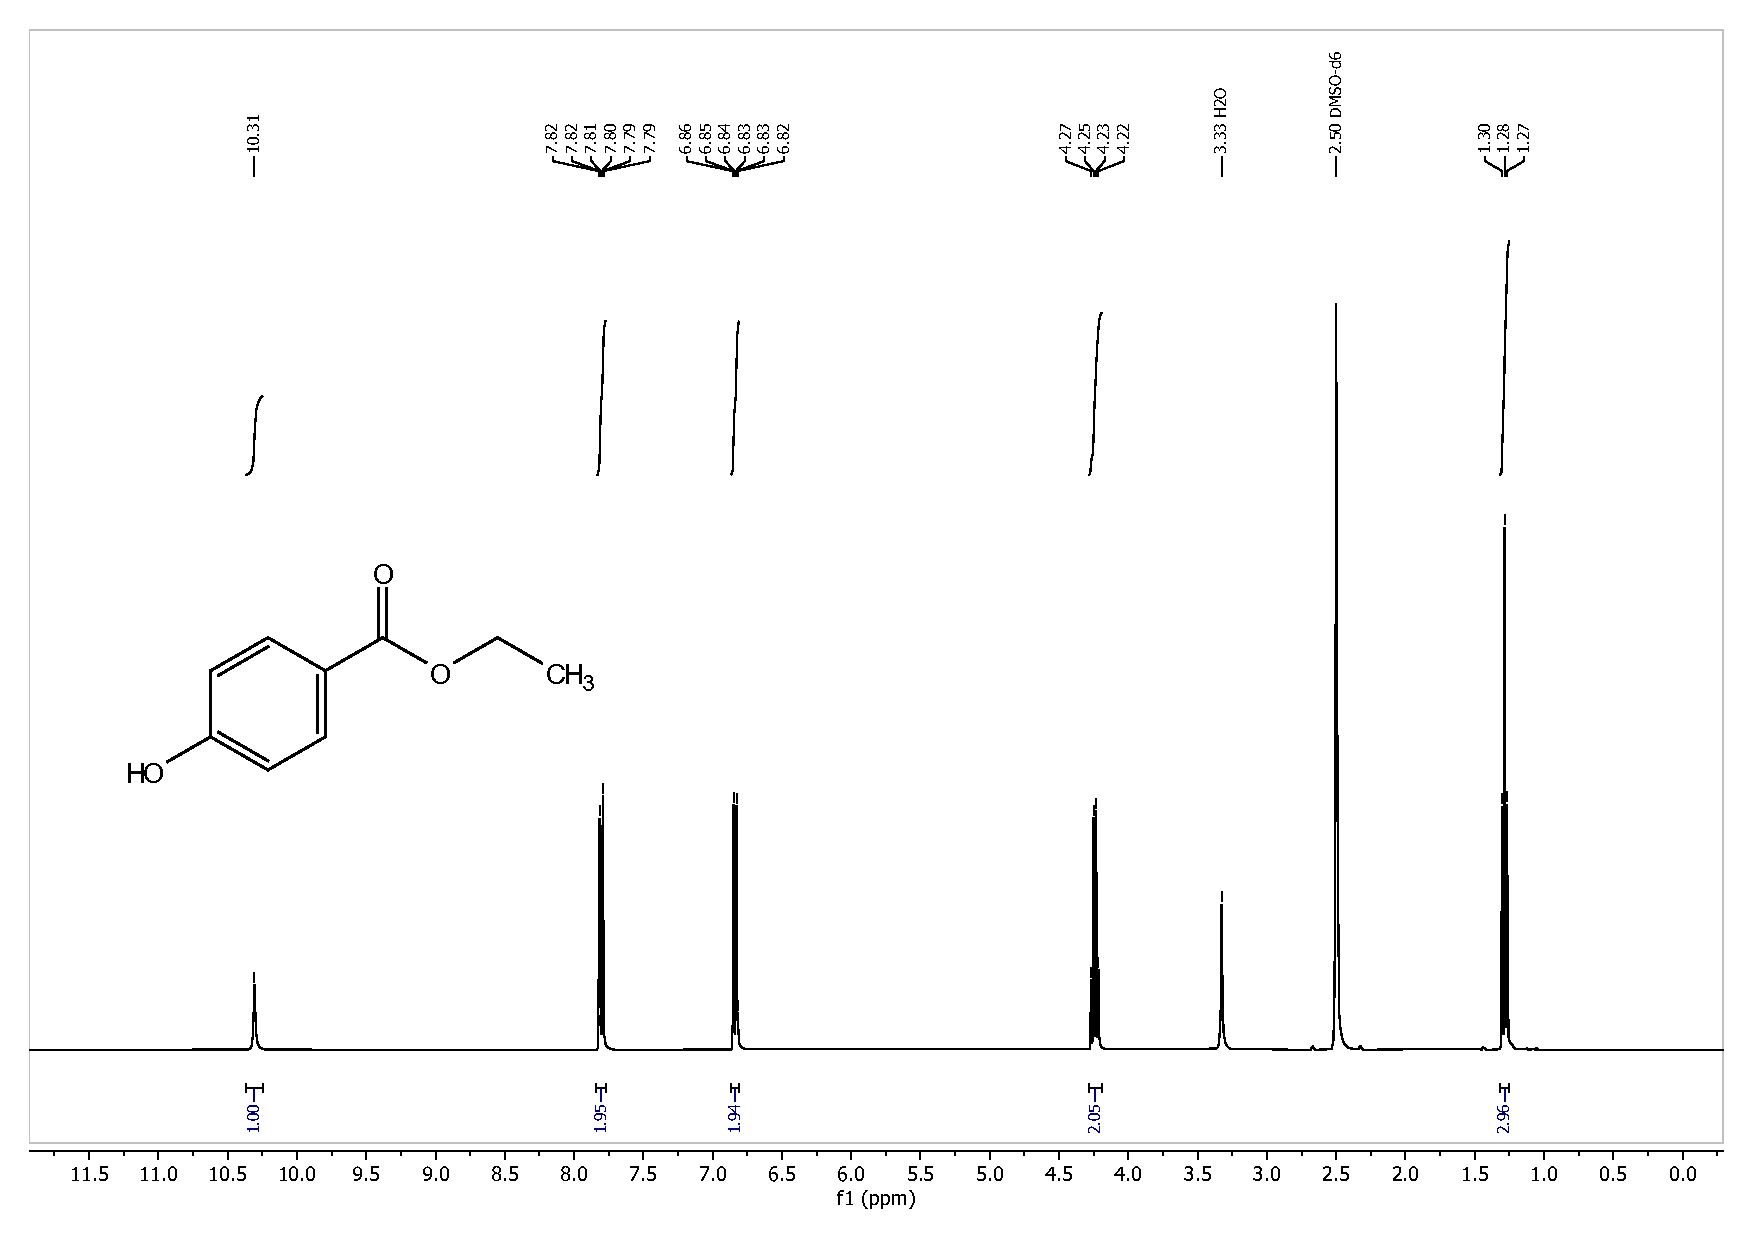
\includegraphics[width=.48\textwidth,page=1]{bilag/ethylnmr}
        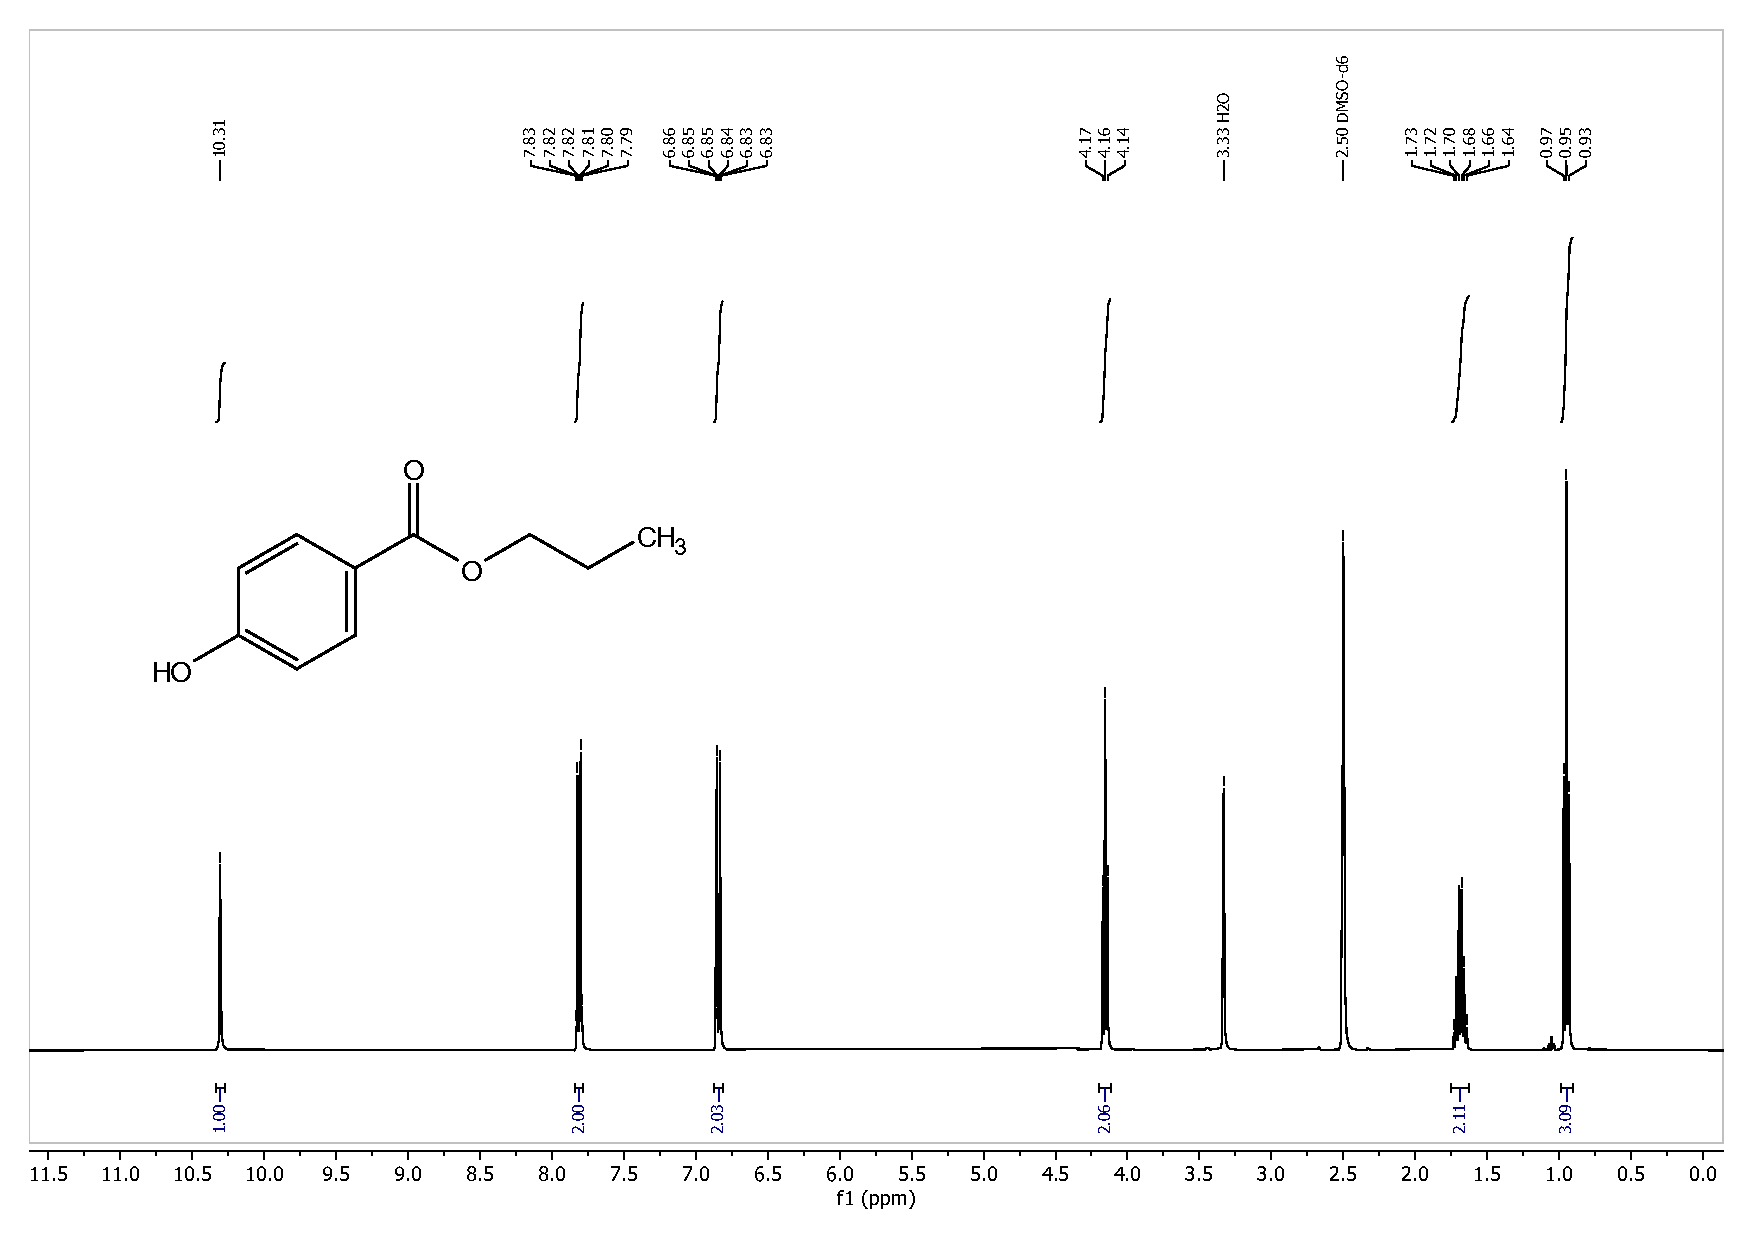
\includegraphics[width=.48\textwidth,page=1]{bilag/propylnmr}
    \end{figure}
    Dette kemiske skift er højere end hvad vi normalt villet forvente for en phenolgruppe (der normalt villet befinde sig omkring det aromatiske område, ligesom ortho- og meta-carbonatomerne). Dette kan begrundes i det benyttede opløsningsmiddel, DMSO-d6, da det har mulighed for at danne hydrogenbindinger med phenolgruppen \parencite{Raym2007}
    \begin{figure}[H]\centering
        \resizebox{\textwidth}{!}{
        \schemestart
        \chemfig{HO-*6(=-=(-COOR)-=-)}
        \+
        \chemfig[-32pt]{S(-[7]CD3)(-[5]CD3)(=[2]O)}
        \arrow(.mid east--.mid west){->}
        \chemfig{O(=[5]S(-[3]CD3)(-[6]CD3))-[2,,,,thick,dotted,red]H(-[1]O-*6(=-=(-COOR)-=-))}
        \schemestop
        }
        \caption{Dannelse af hydrogenbinding mellem DMSO-d6 og vilkårlig paraben.}
    \end{figure}
    Umiddelbart passer H--NMR--spektrene for begge produkter meget godt med hvad vi villet forvente i teorien-- samt ved sammenligning med praktiske spektre udarbejdet af laboratorier, og der vurderes derfor sandsynligt at det dannede produkt er hvad det burde være grundet NMR--spektroskopis høje selektivitet.
    \begin{figure}[H]\centering
        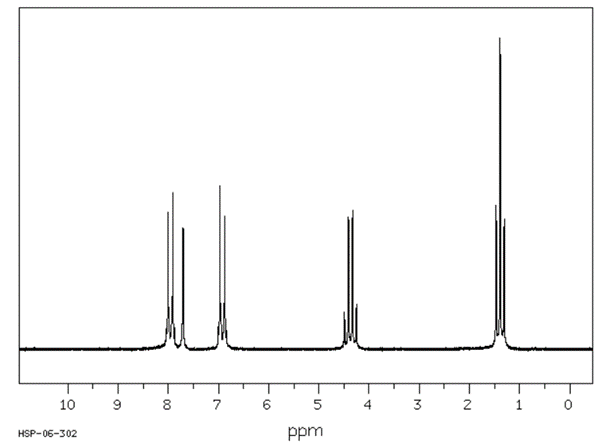
\includegraphics[width=.48\linewidth]{billeder/teonmrethyl}
        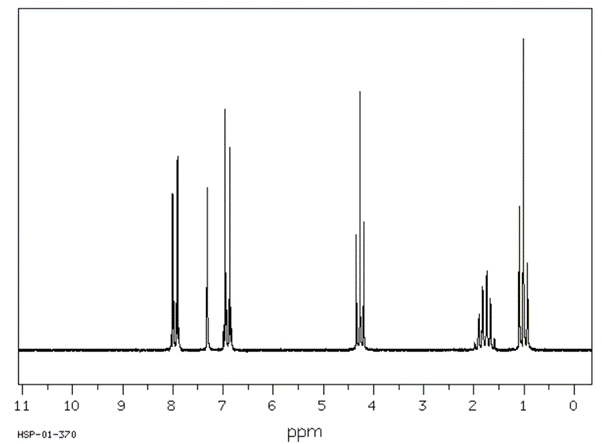
\includegraphics[width=.48\linewidth]{billeder/teonmrpropyl}
        \caption{Praktiske H--NMR--spektre for hhv.\ ethyl-- og propylparaben \parencite{SDBS}}
    \end{figure}

    \subsection{IR--spektroskopi}
    Først undersøges IR--spektret dannet for ethylparaben for at forsøge at identificerer funktionelle grupper vi villet forvente at være tilstede.
    \begin{figure}[H]
        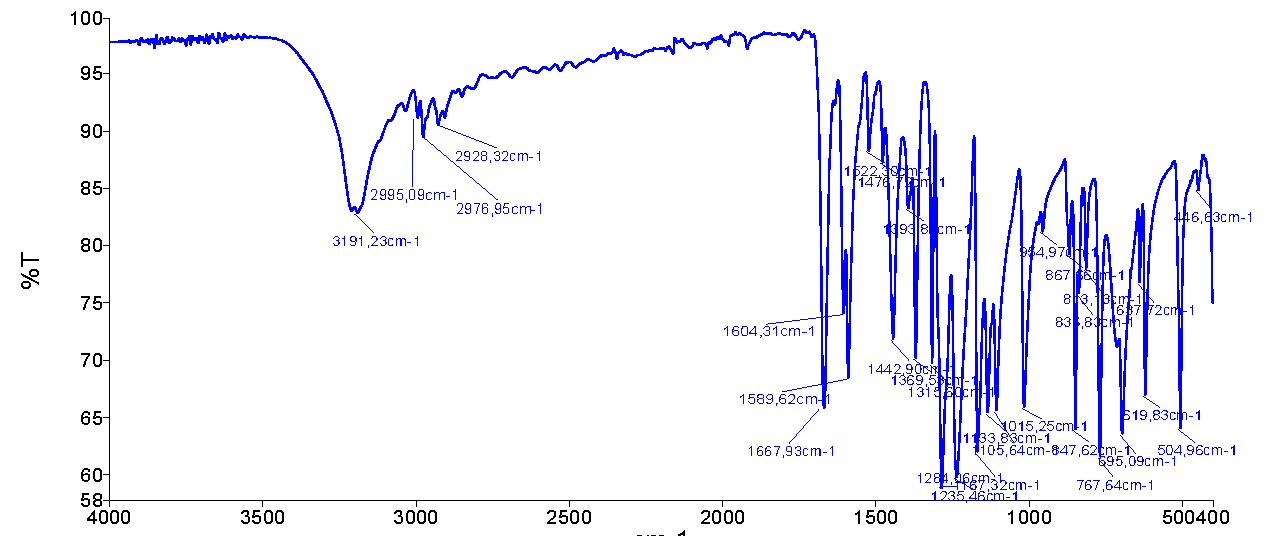
\includegraphics[width=\linewidth]{bilag/ethylir}
        \caption{IR--spektra for dannet ethylparaben.}
    \end{figure}
    Der ses tydeligt den karakteristiske bøjninger der korresponderer til hydroxy--grupper, hvilket giver god mening da molekylet indeholder sådan en. Derudover observeres det at der er et par udsvingninger i området svarende til C--H--bindinger hvilket igen giver mening jf.\ molekylstrukturen.
    \begin{figure}[H]
        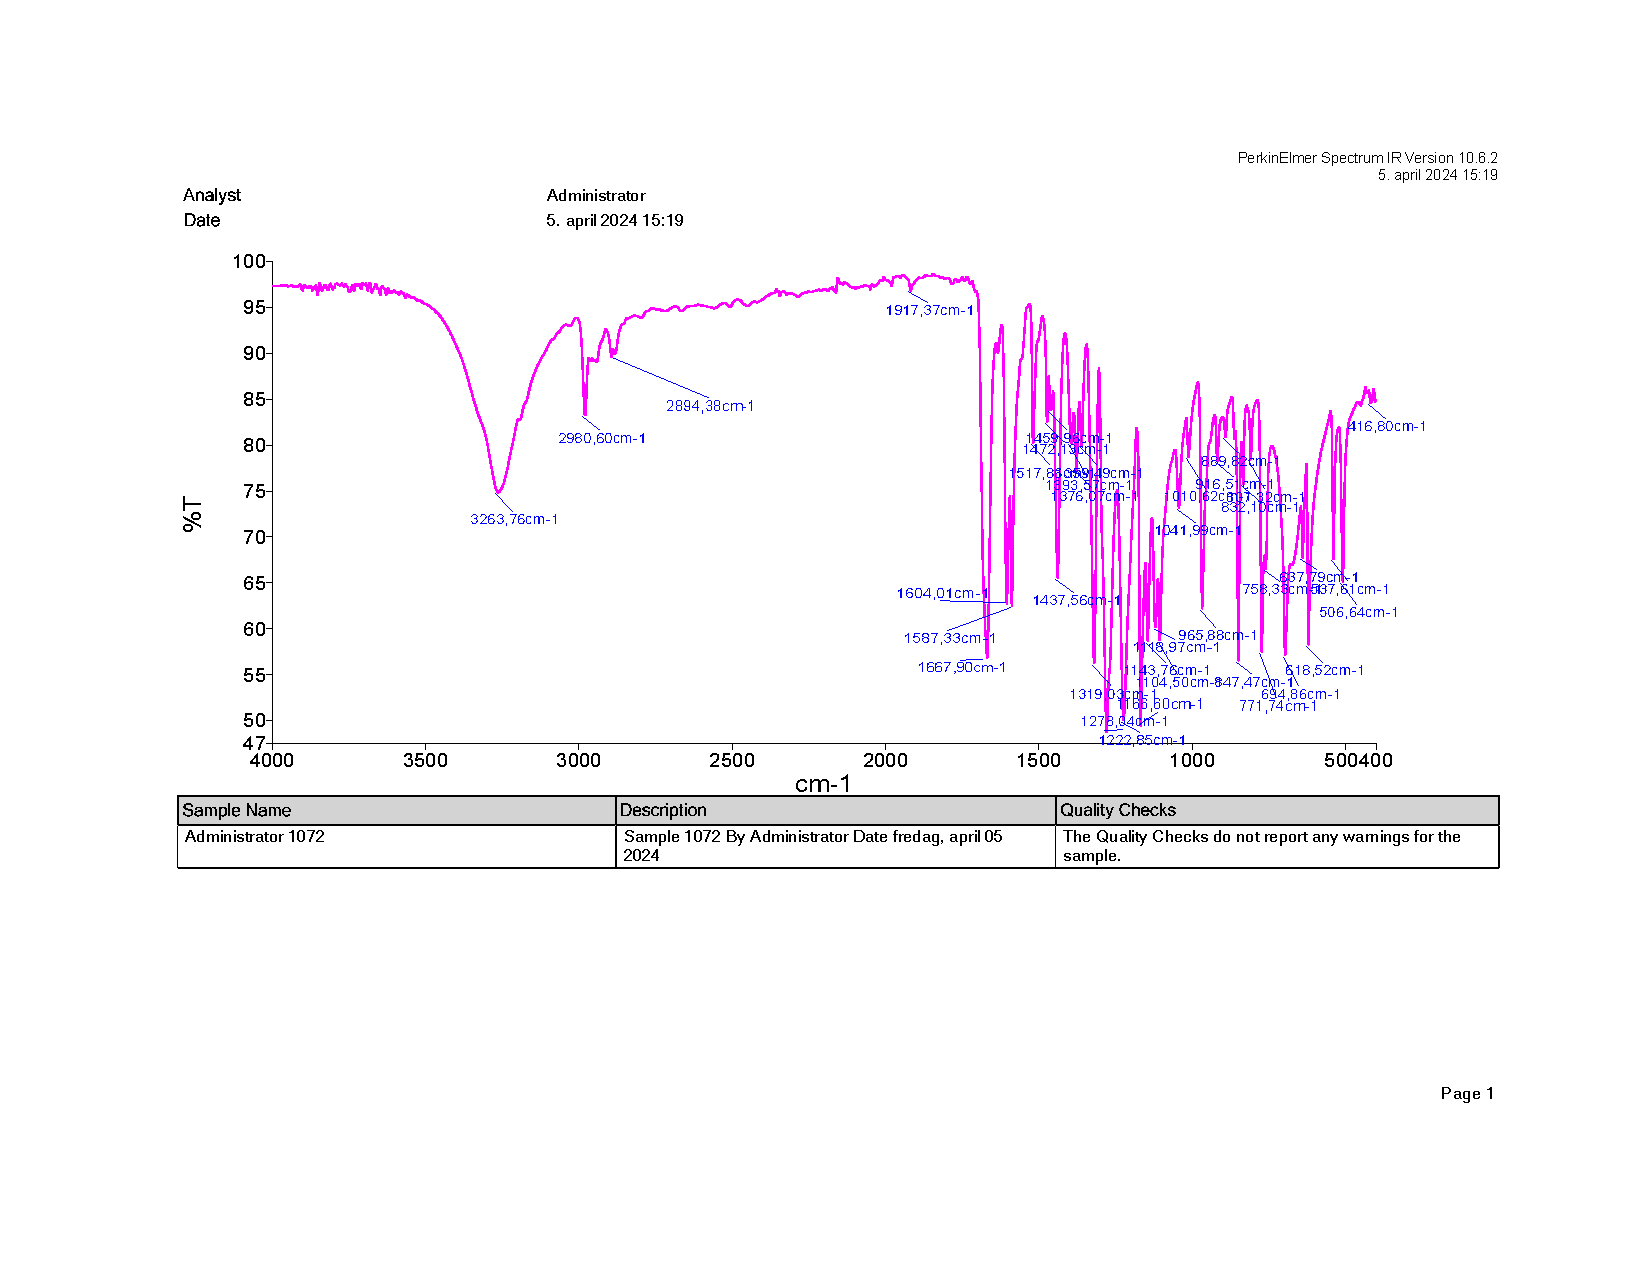
\includegraphics[width=\linewidth]{bilag/propylir}
        \caption{IR--spektra for dannet propylparaben.}
    \end{figure}
    Igen ses bøjningen korresponderende til hydroxy--gruppen samt bøjninger i området der associeres med C--H bindinger. Der er meget få betydningsfulde forskelle mellem spektrene, da molekylerne ligner hinanden meget og indeholder de samme funktionelle grupper.

    Samtidigt er det også muligt at samligne de dannede spektre med teoretiske spektre fundet i databaser:
    \begin{figure}[H]
        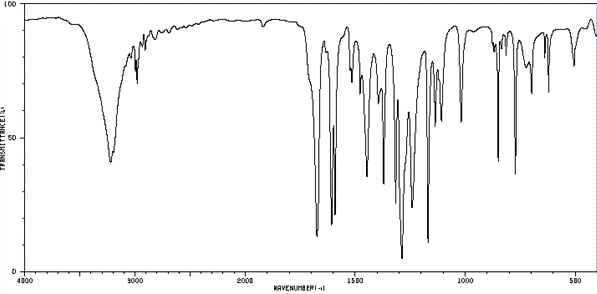
\includegraphics[width=.48\linewidth]{billeder/irethyl}
        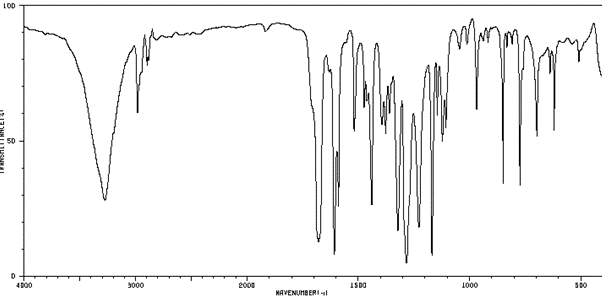
\includegraphics[width=.48\linewidth]{billeder/irpropyl}
        \caption{Teoretisk IR--spektre for hhv.\ ethyl-- og propylparaben.}
    \end{figure}
    Disse stemmer også overens med dem produceret af Aarhus Universitet, da vi observerer O--H strækningen i dem begge, samt forskellenene i ``støjmængden'' ved området svarende til C--H bindinger. Denne enshed mellem spektrene for produktet dannet ved syntese og dem for et kendt rent produkt medfører større sikkerhed på at det korrekte produkt er dannet.

    \subsection{Hæmningsforsøg}
    \subsubsection{Agar--diffusion}
    Efter agarpladerne har stået natten over, observeres de for at bestemme den hæmmende radius fra hver papirdisk.
    \begin{figure}[H]\centering
        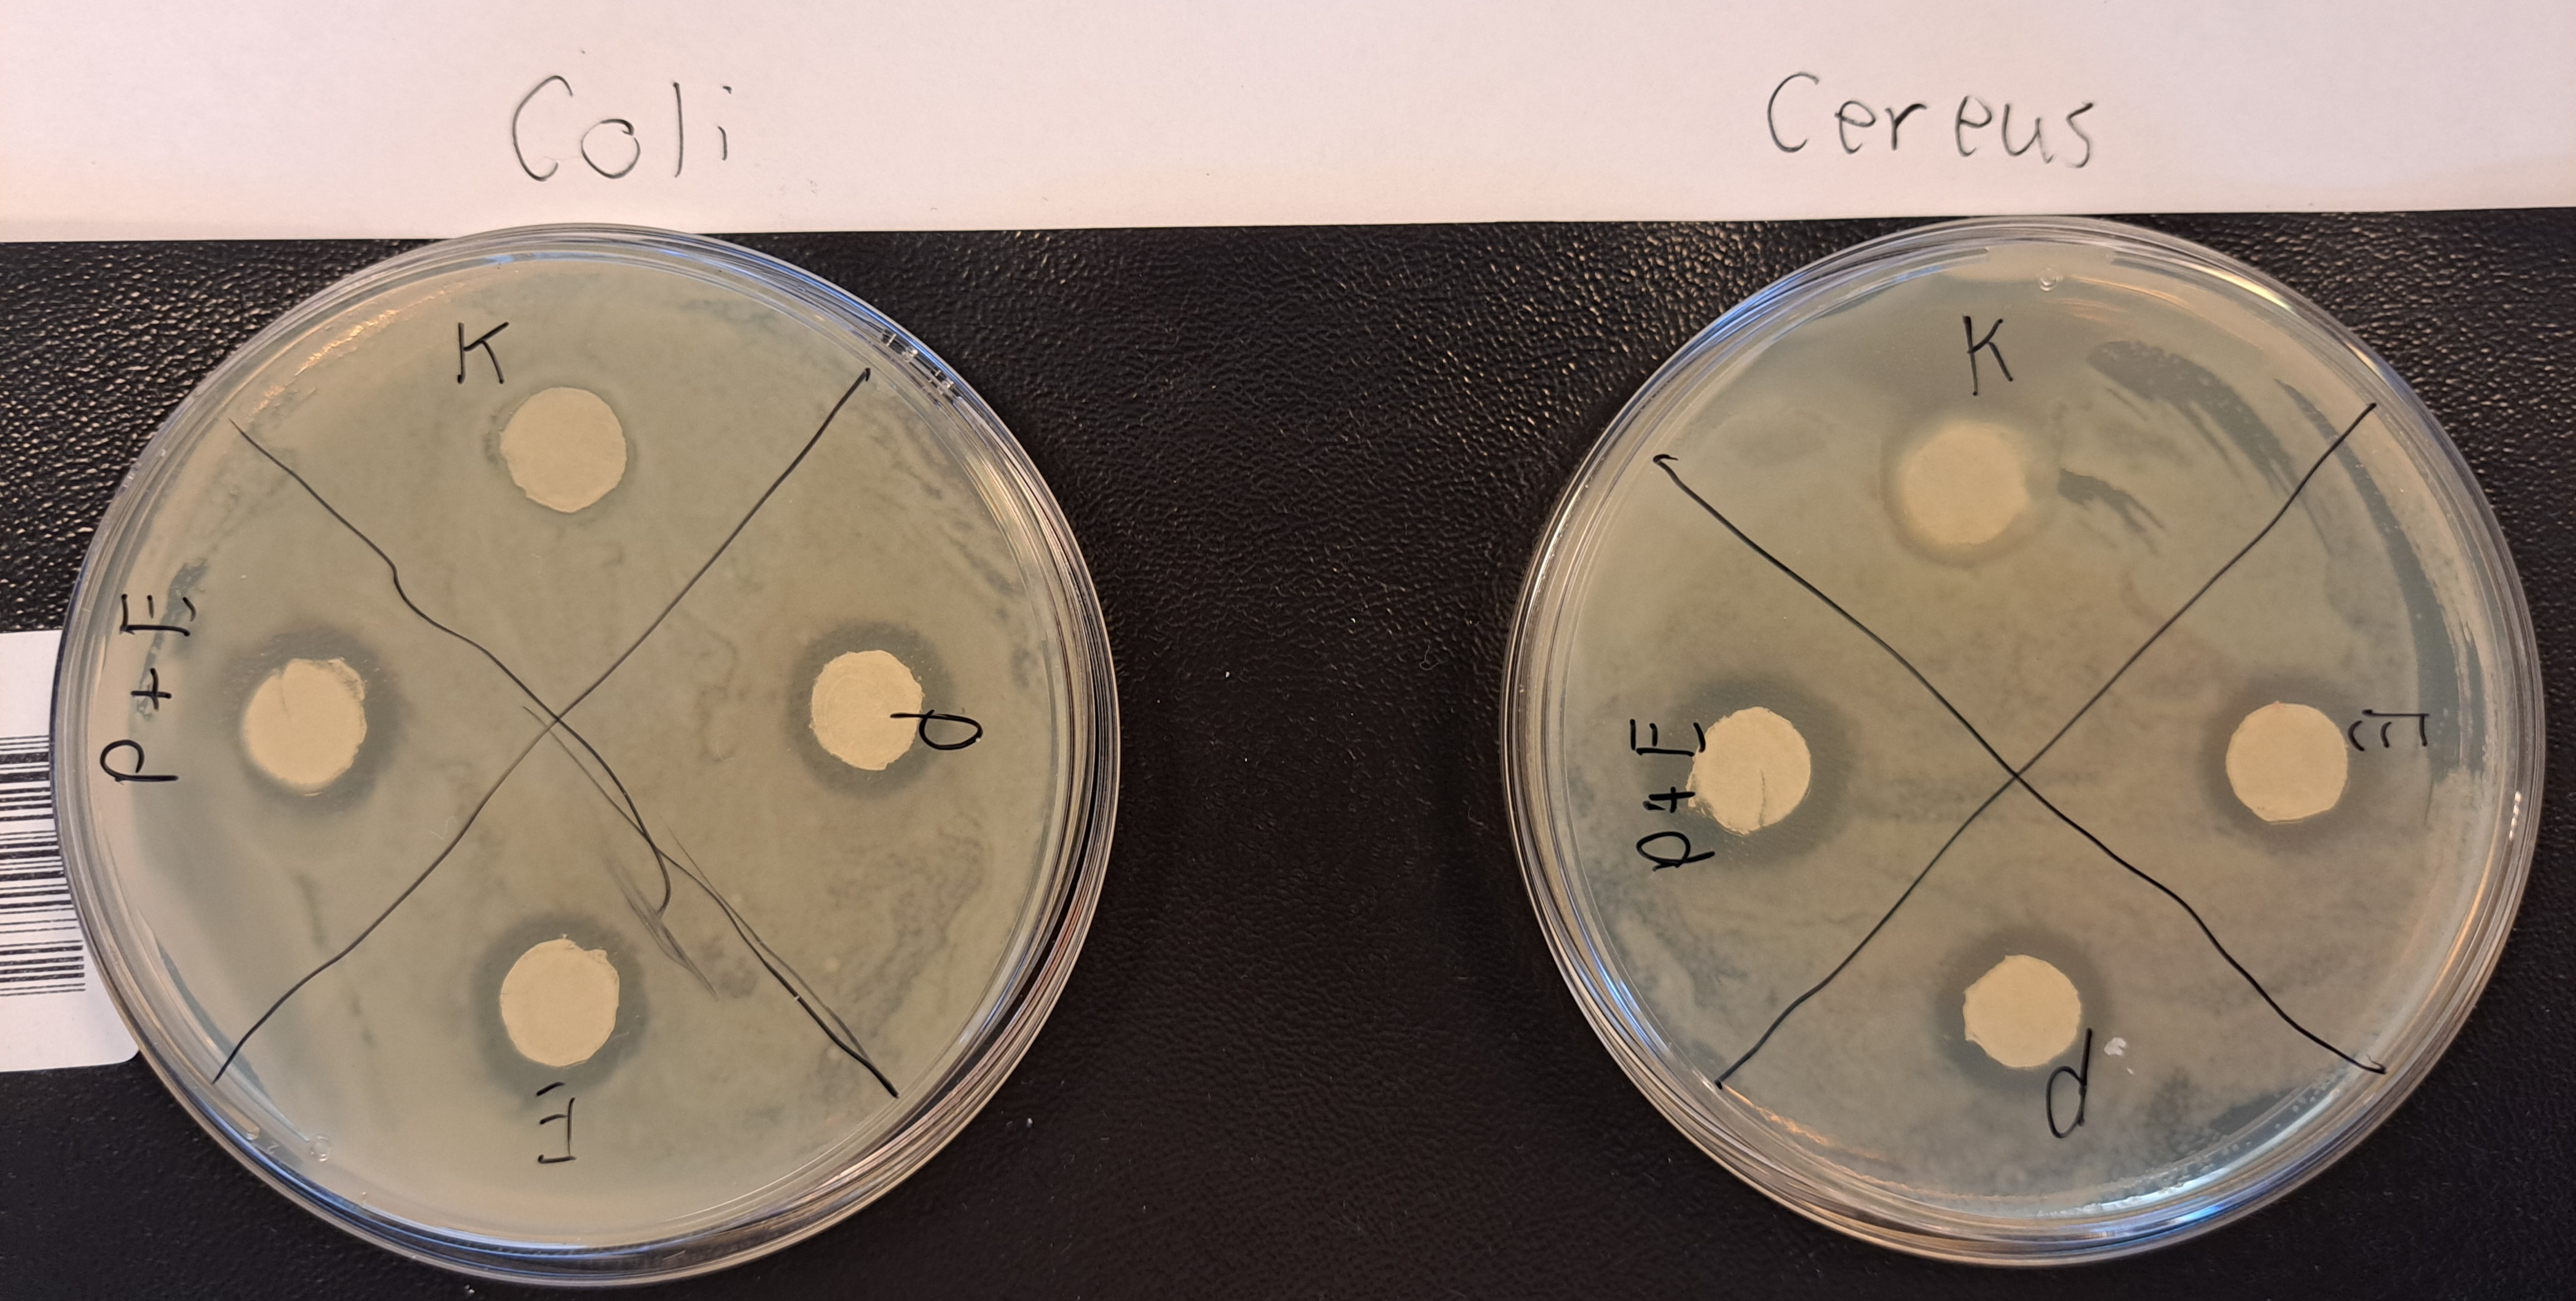
\includegraphics[width=\textwidth]{billeder/agar2}
        \caption{Agarplader efter inkubering natten over.}
    \end{figure}
    For cereuskolonien fik vi at hæmning ved alle diskene væddet i parabenopløsning, og ingen hæmning ved kontrollen. Det er derfor relativt sikkert at ethanolen er fordampet, og at dets indvirkning derfor har været minimal:
    \begin{figure}[H]\centering
        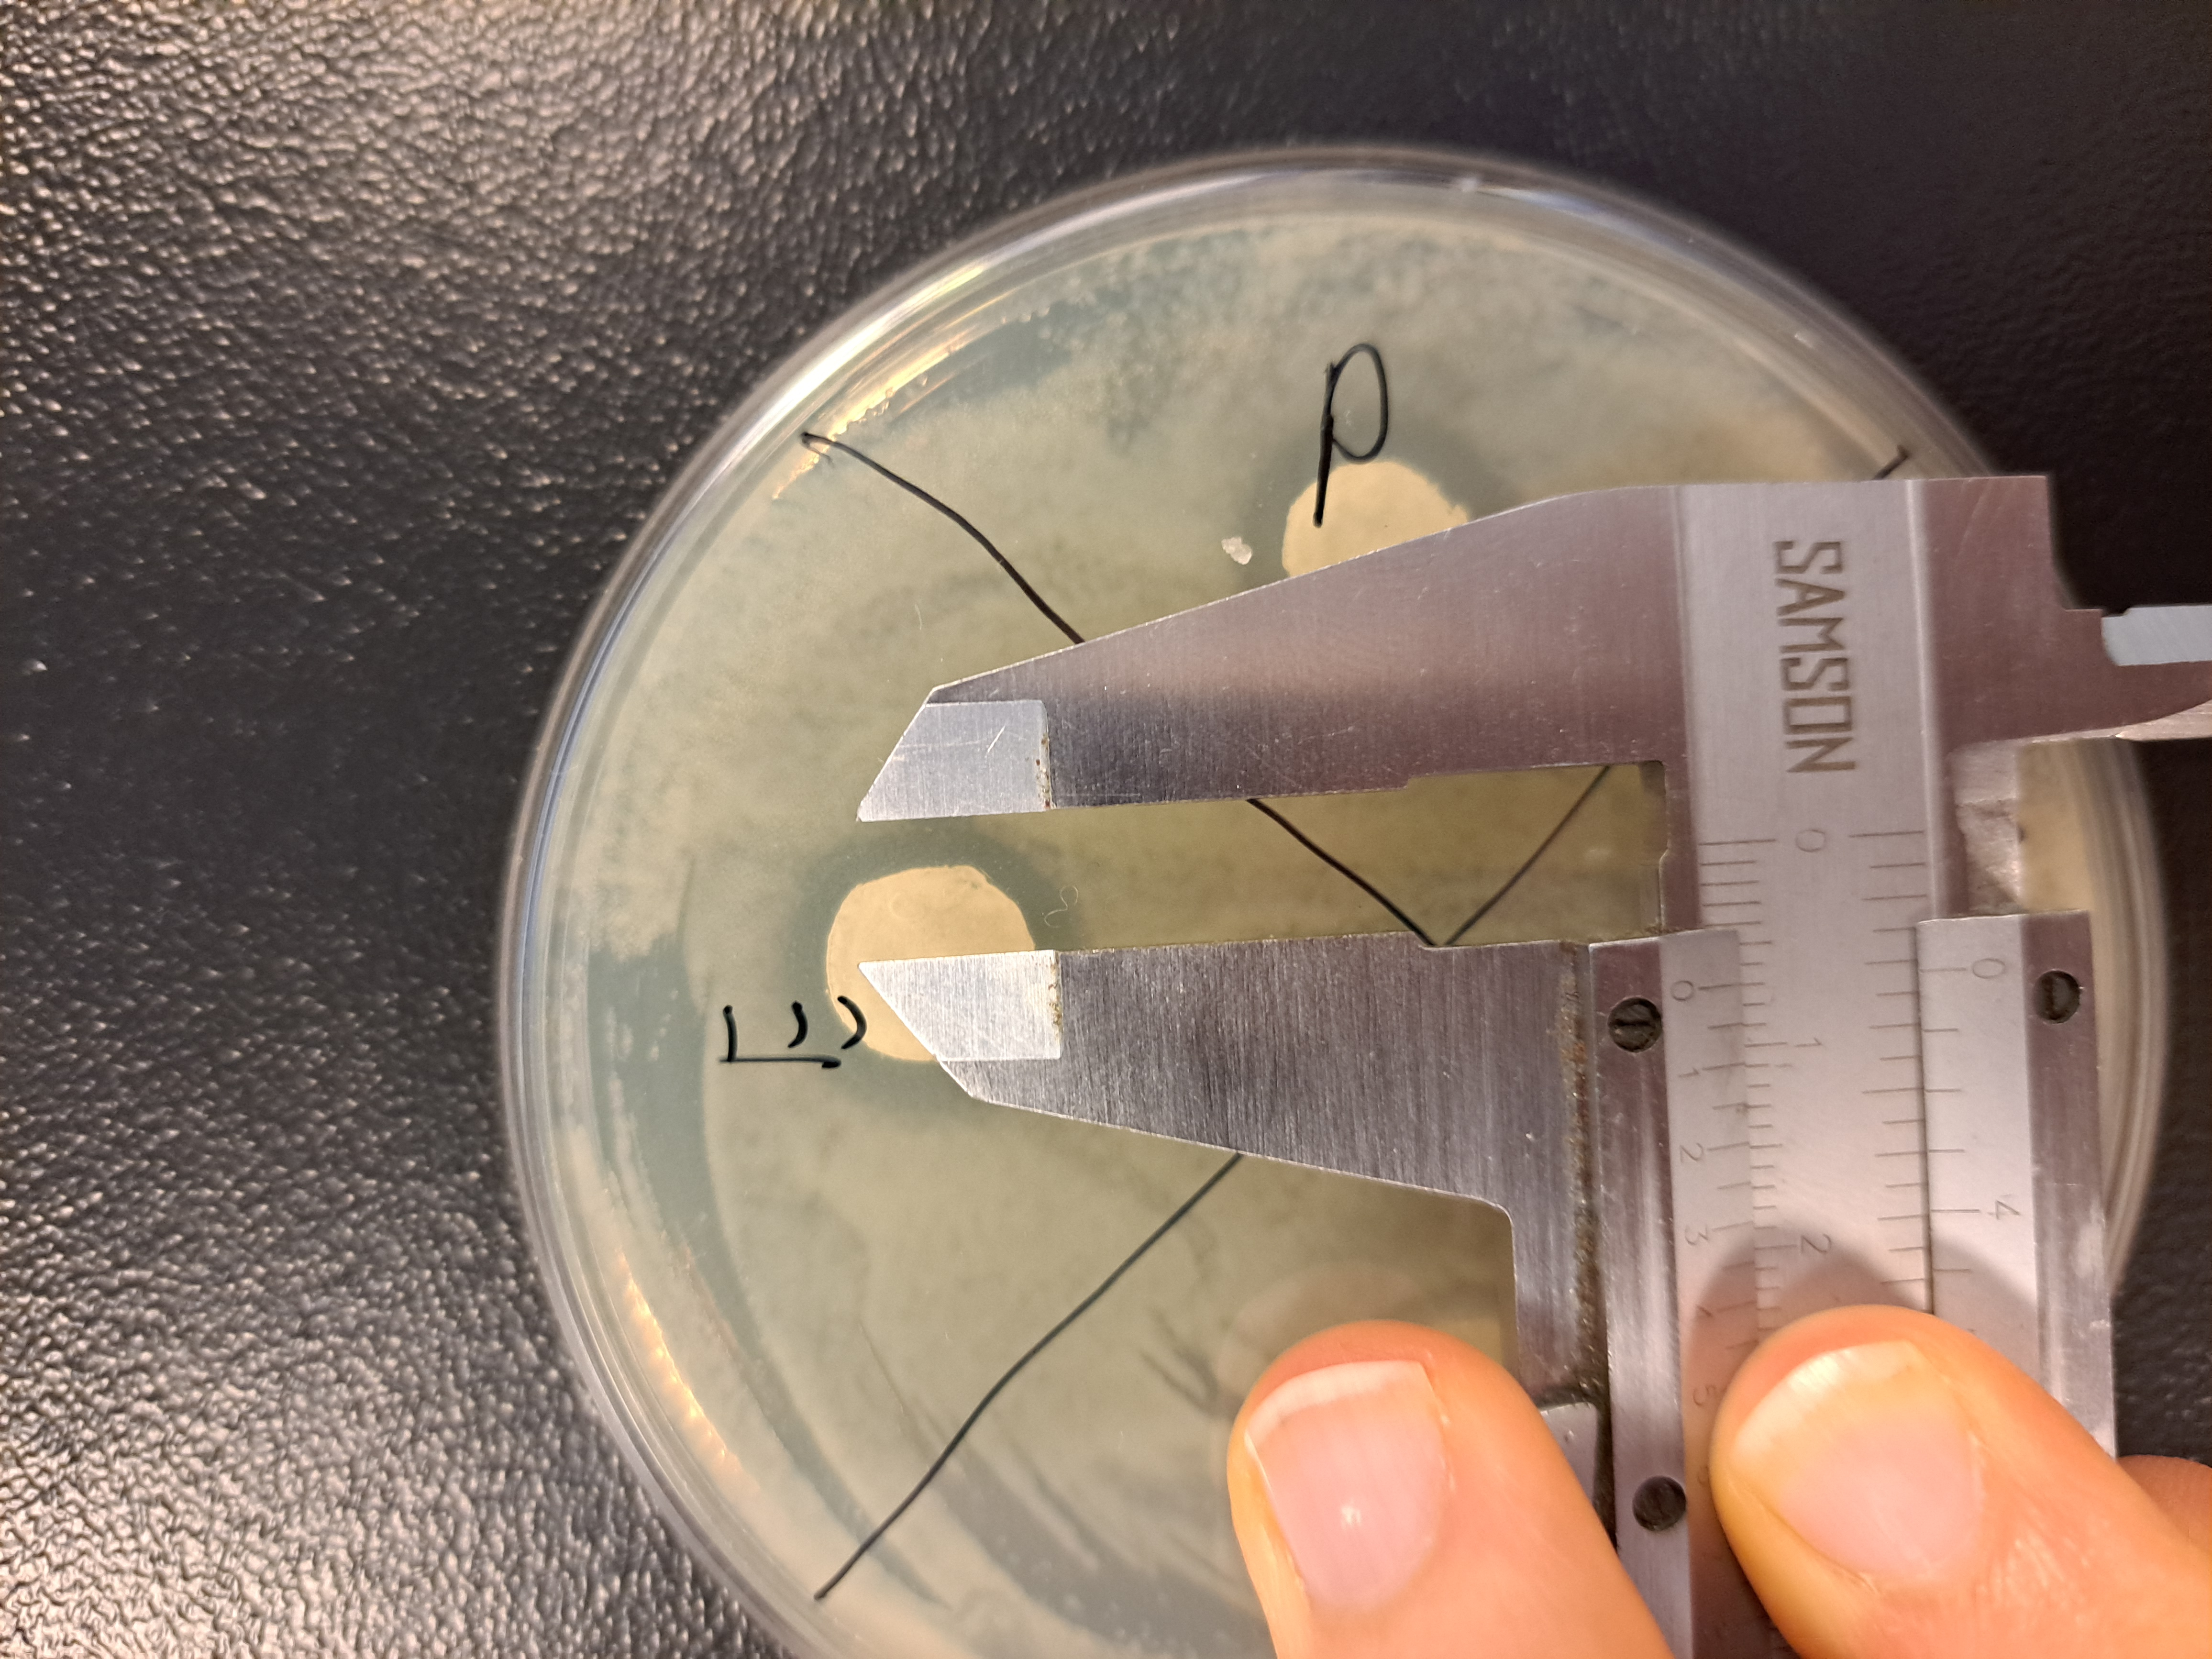
\includegraphics[width=.32\textwidth]{billeder/cereuse}
        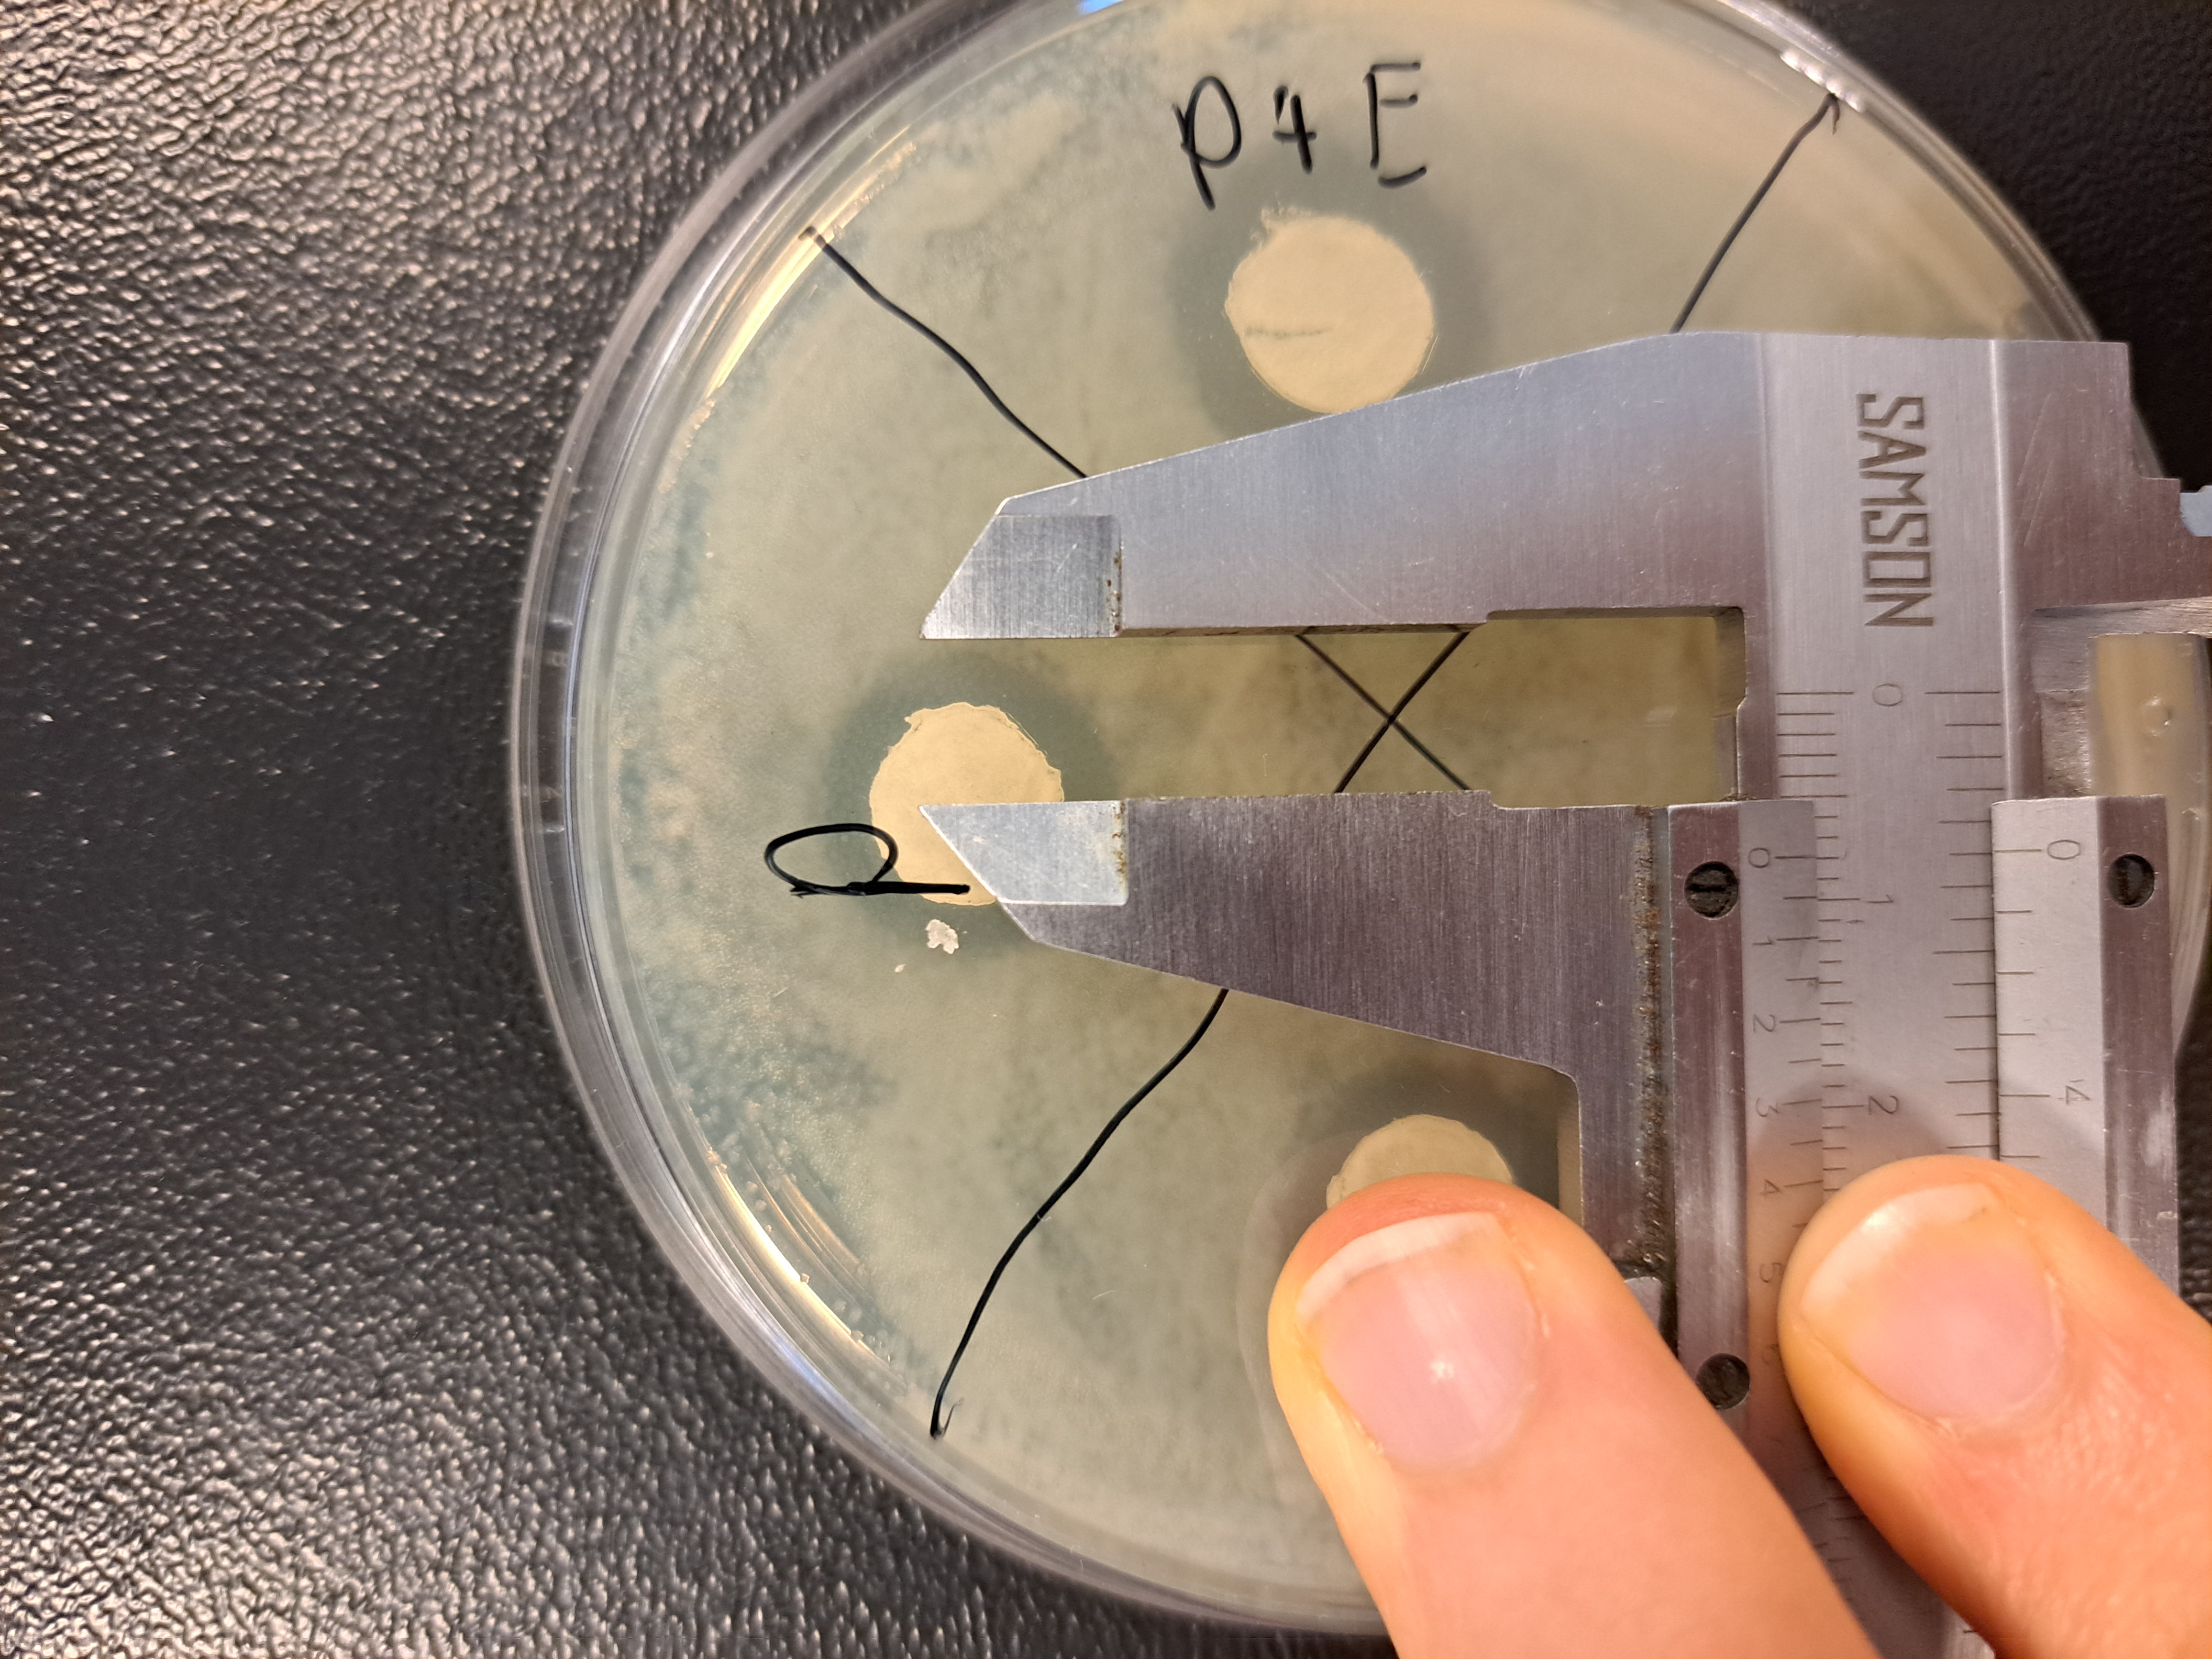
\includegraphics[width=.32\textwidth]{billeder/cereusp}
        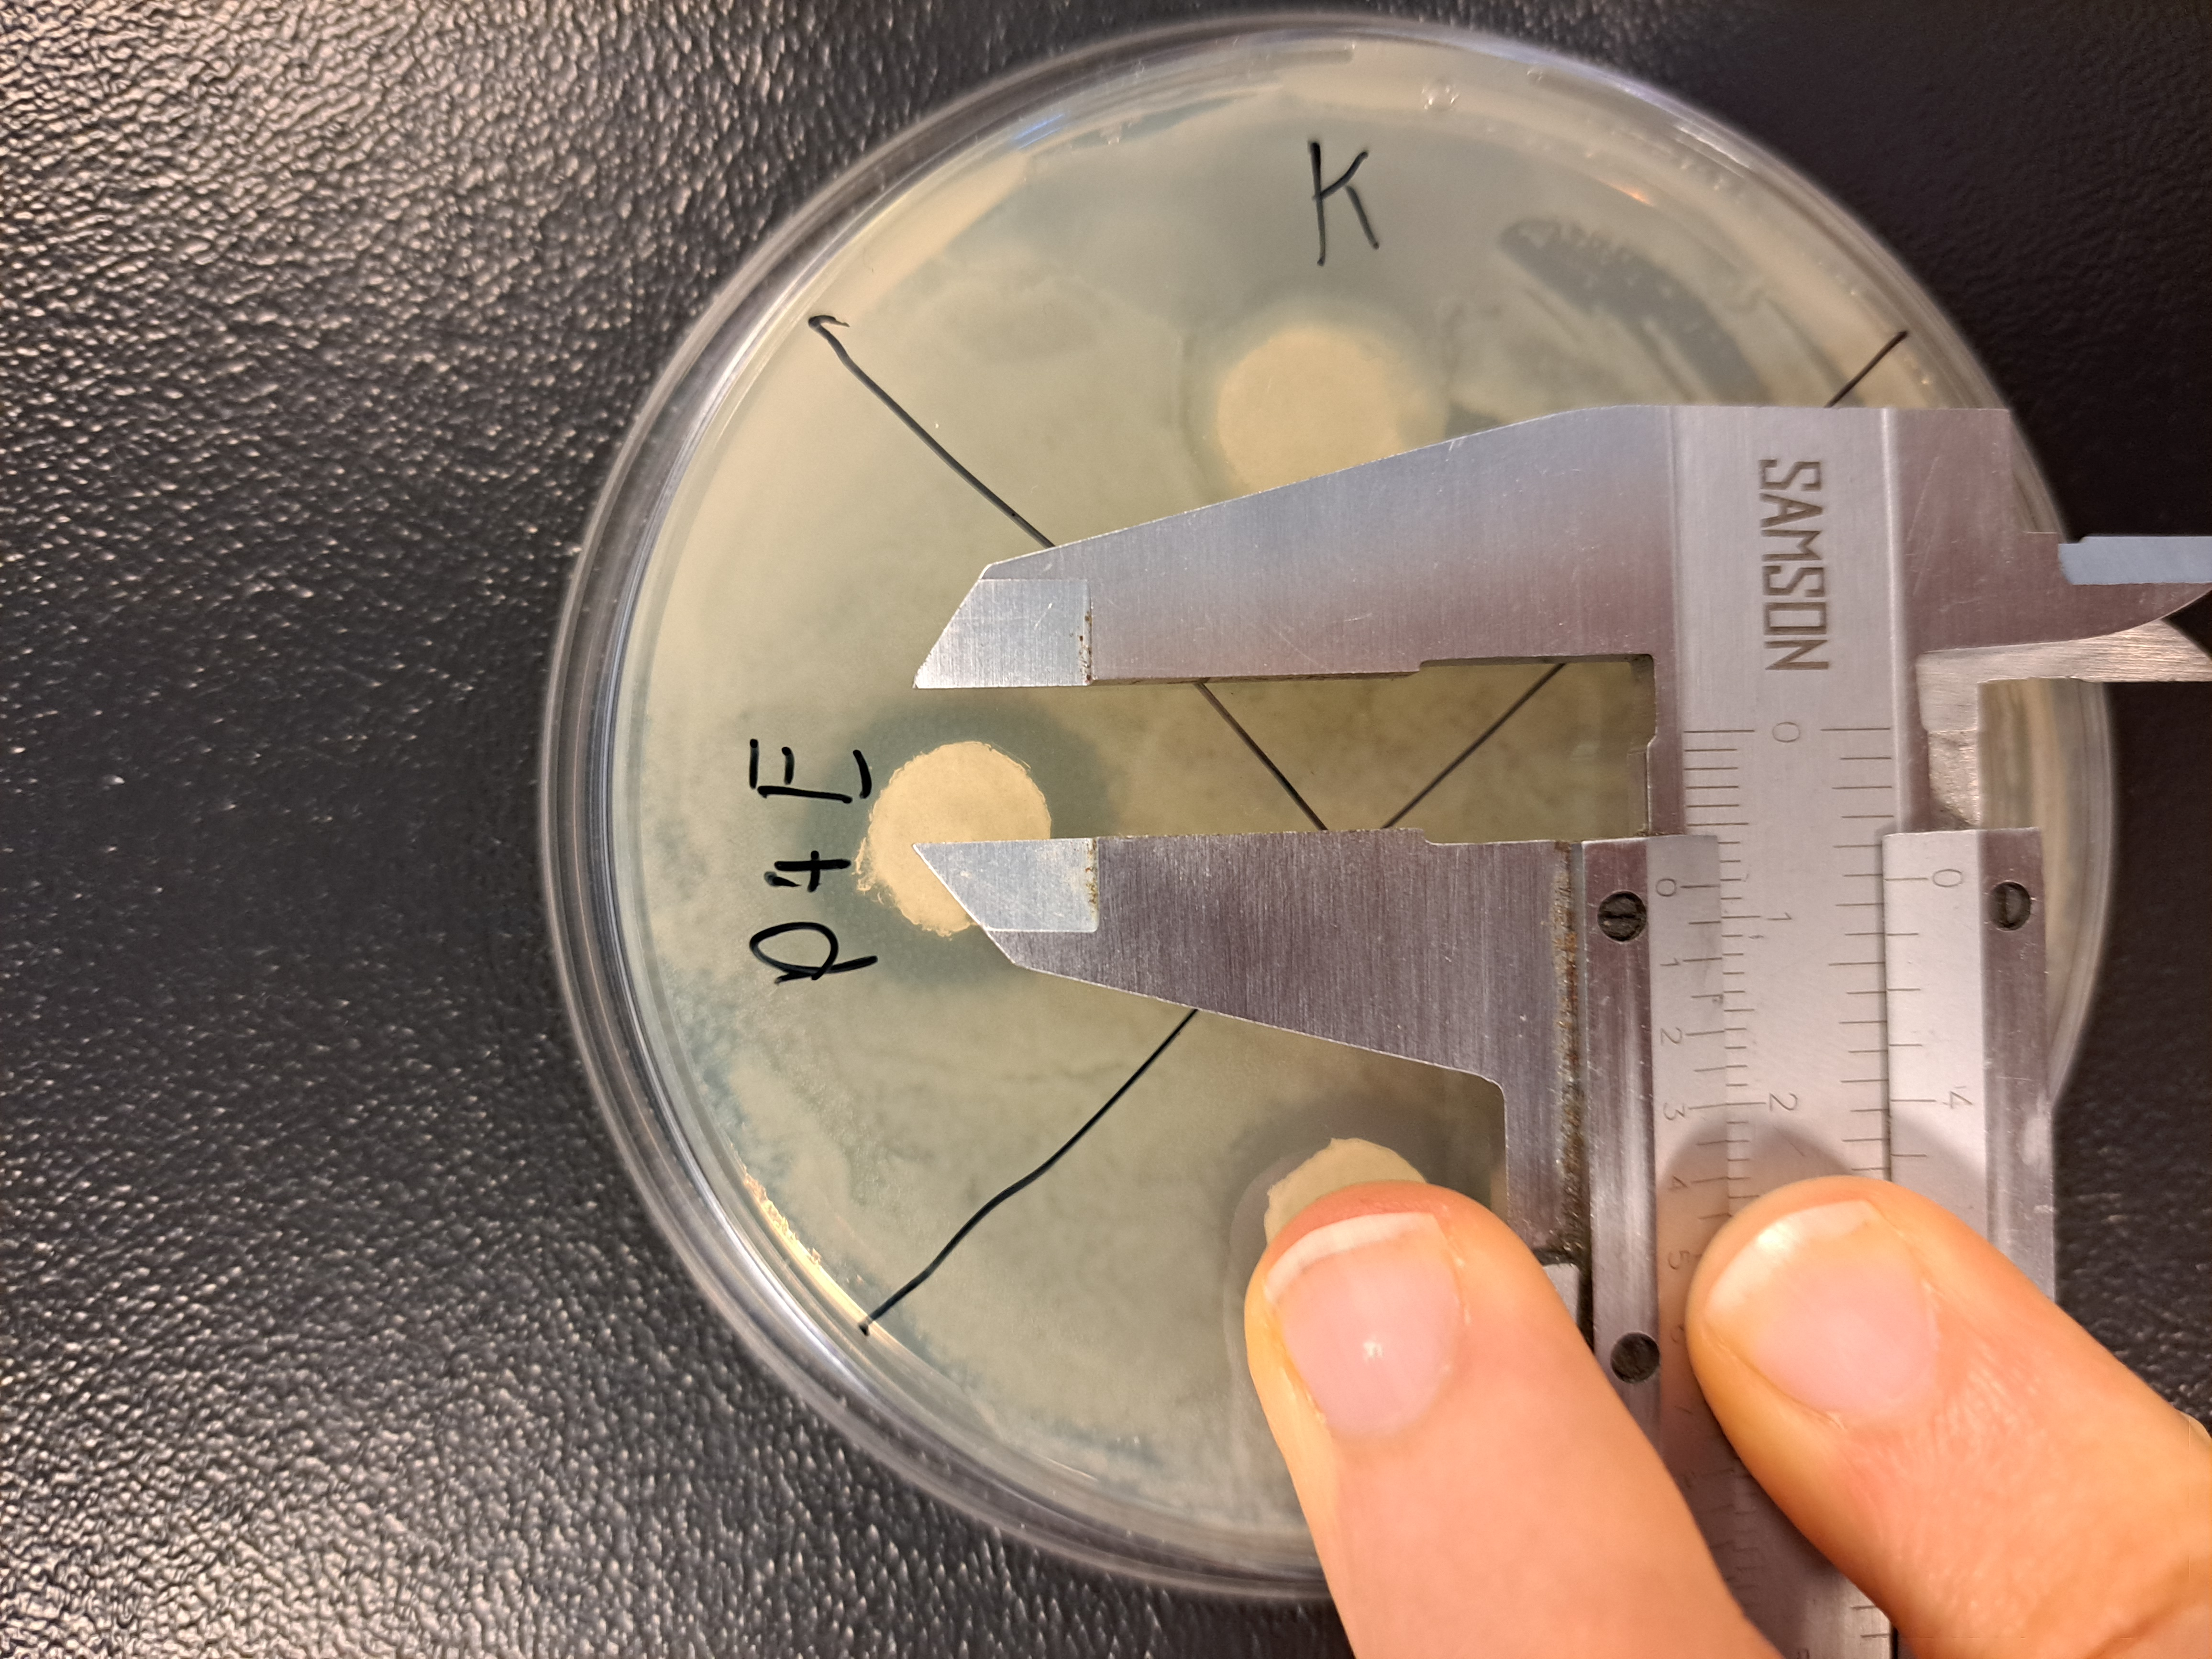
\includegraphics[width=.32\textwidth]{billeder/cereuspe}
        \caption{Hæmningsradier for cereuskolonien.}
    \end{figure}
    Det samme observeredes for colikolonien:
    \begin{figure}[H]\centering
        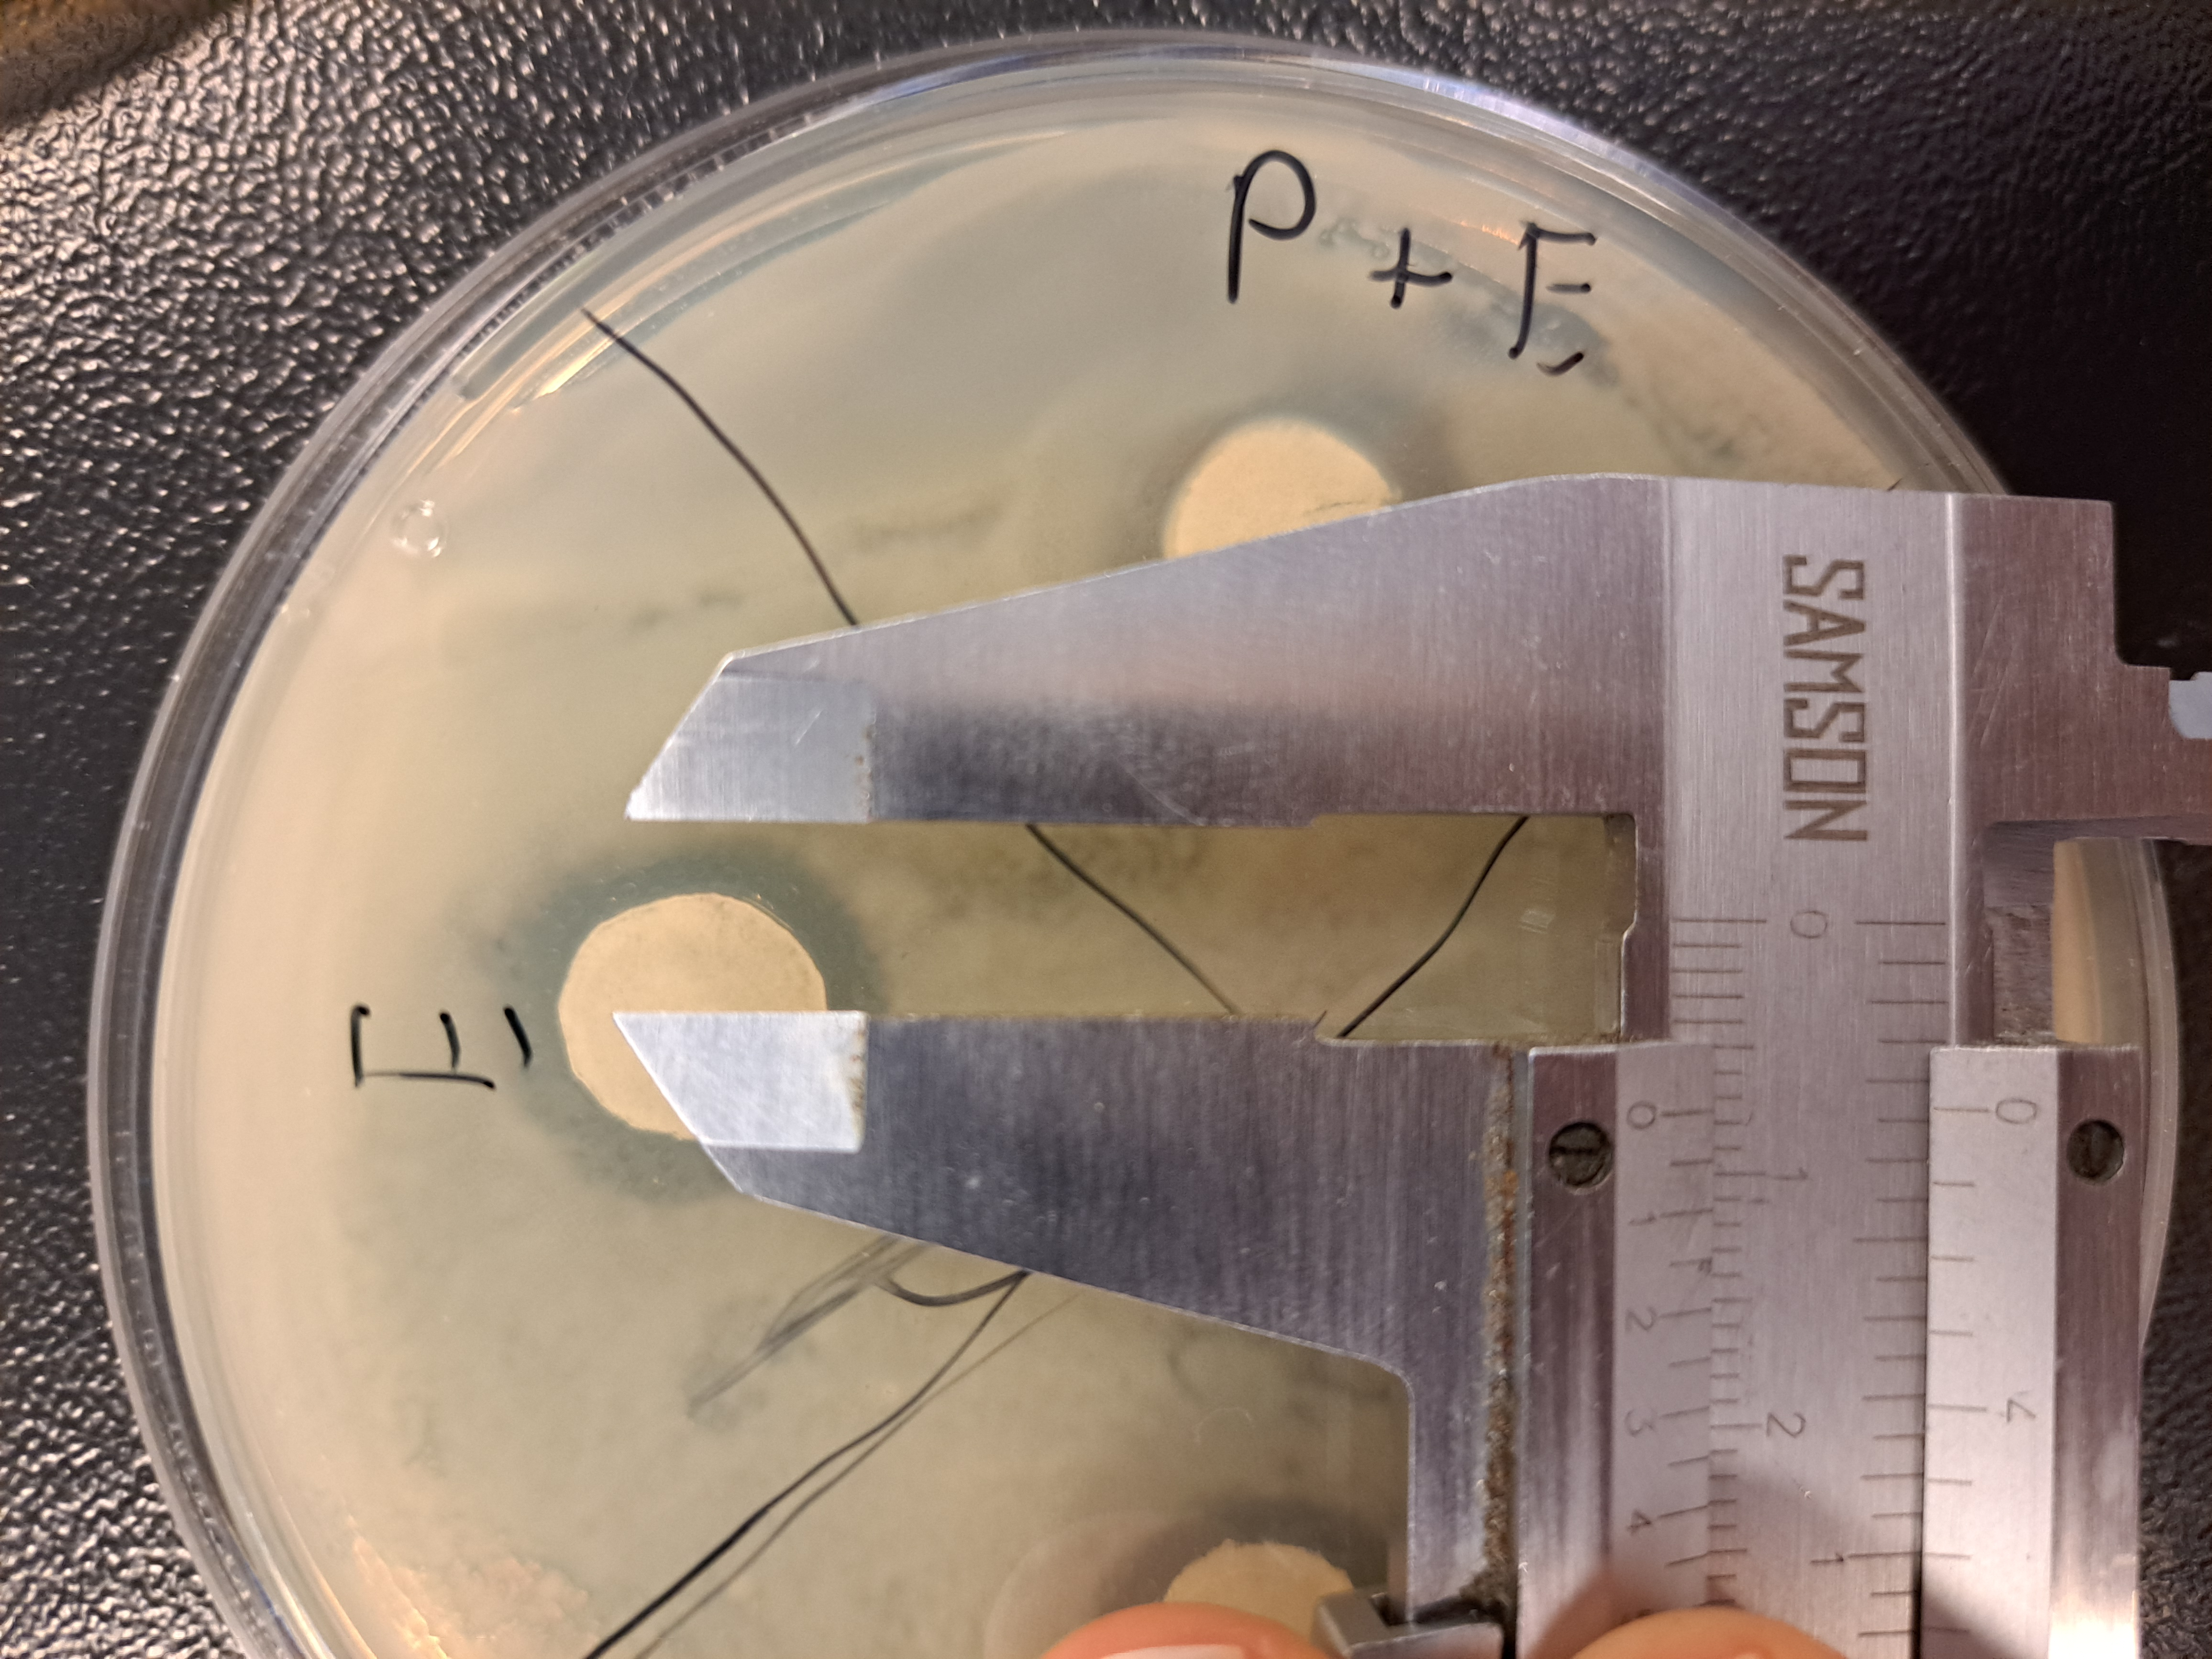
\includegraphics[width=.32\textwidth]{billeder/colie}
        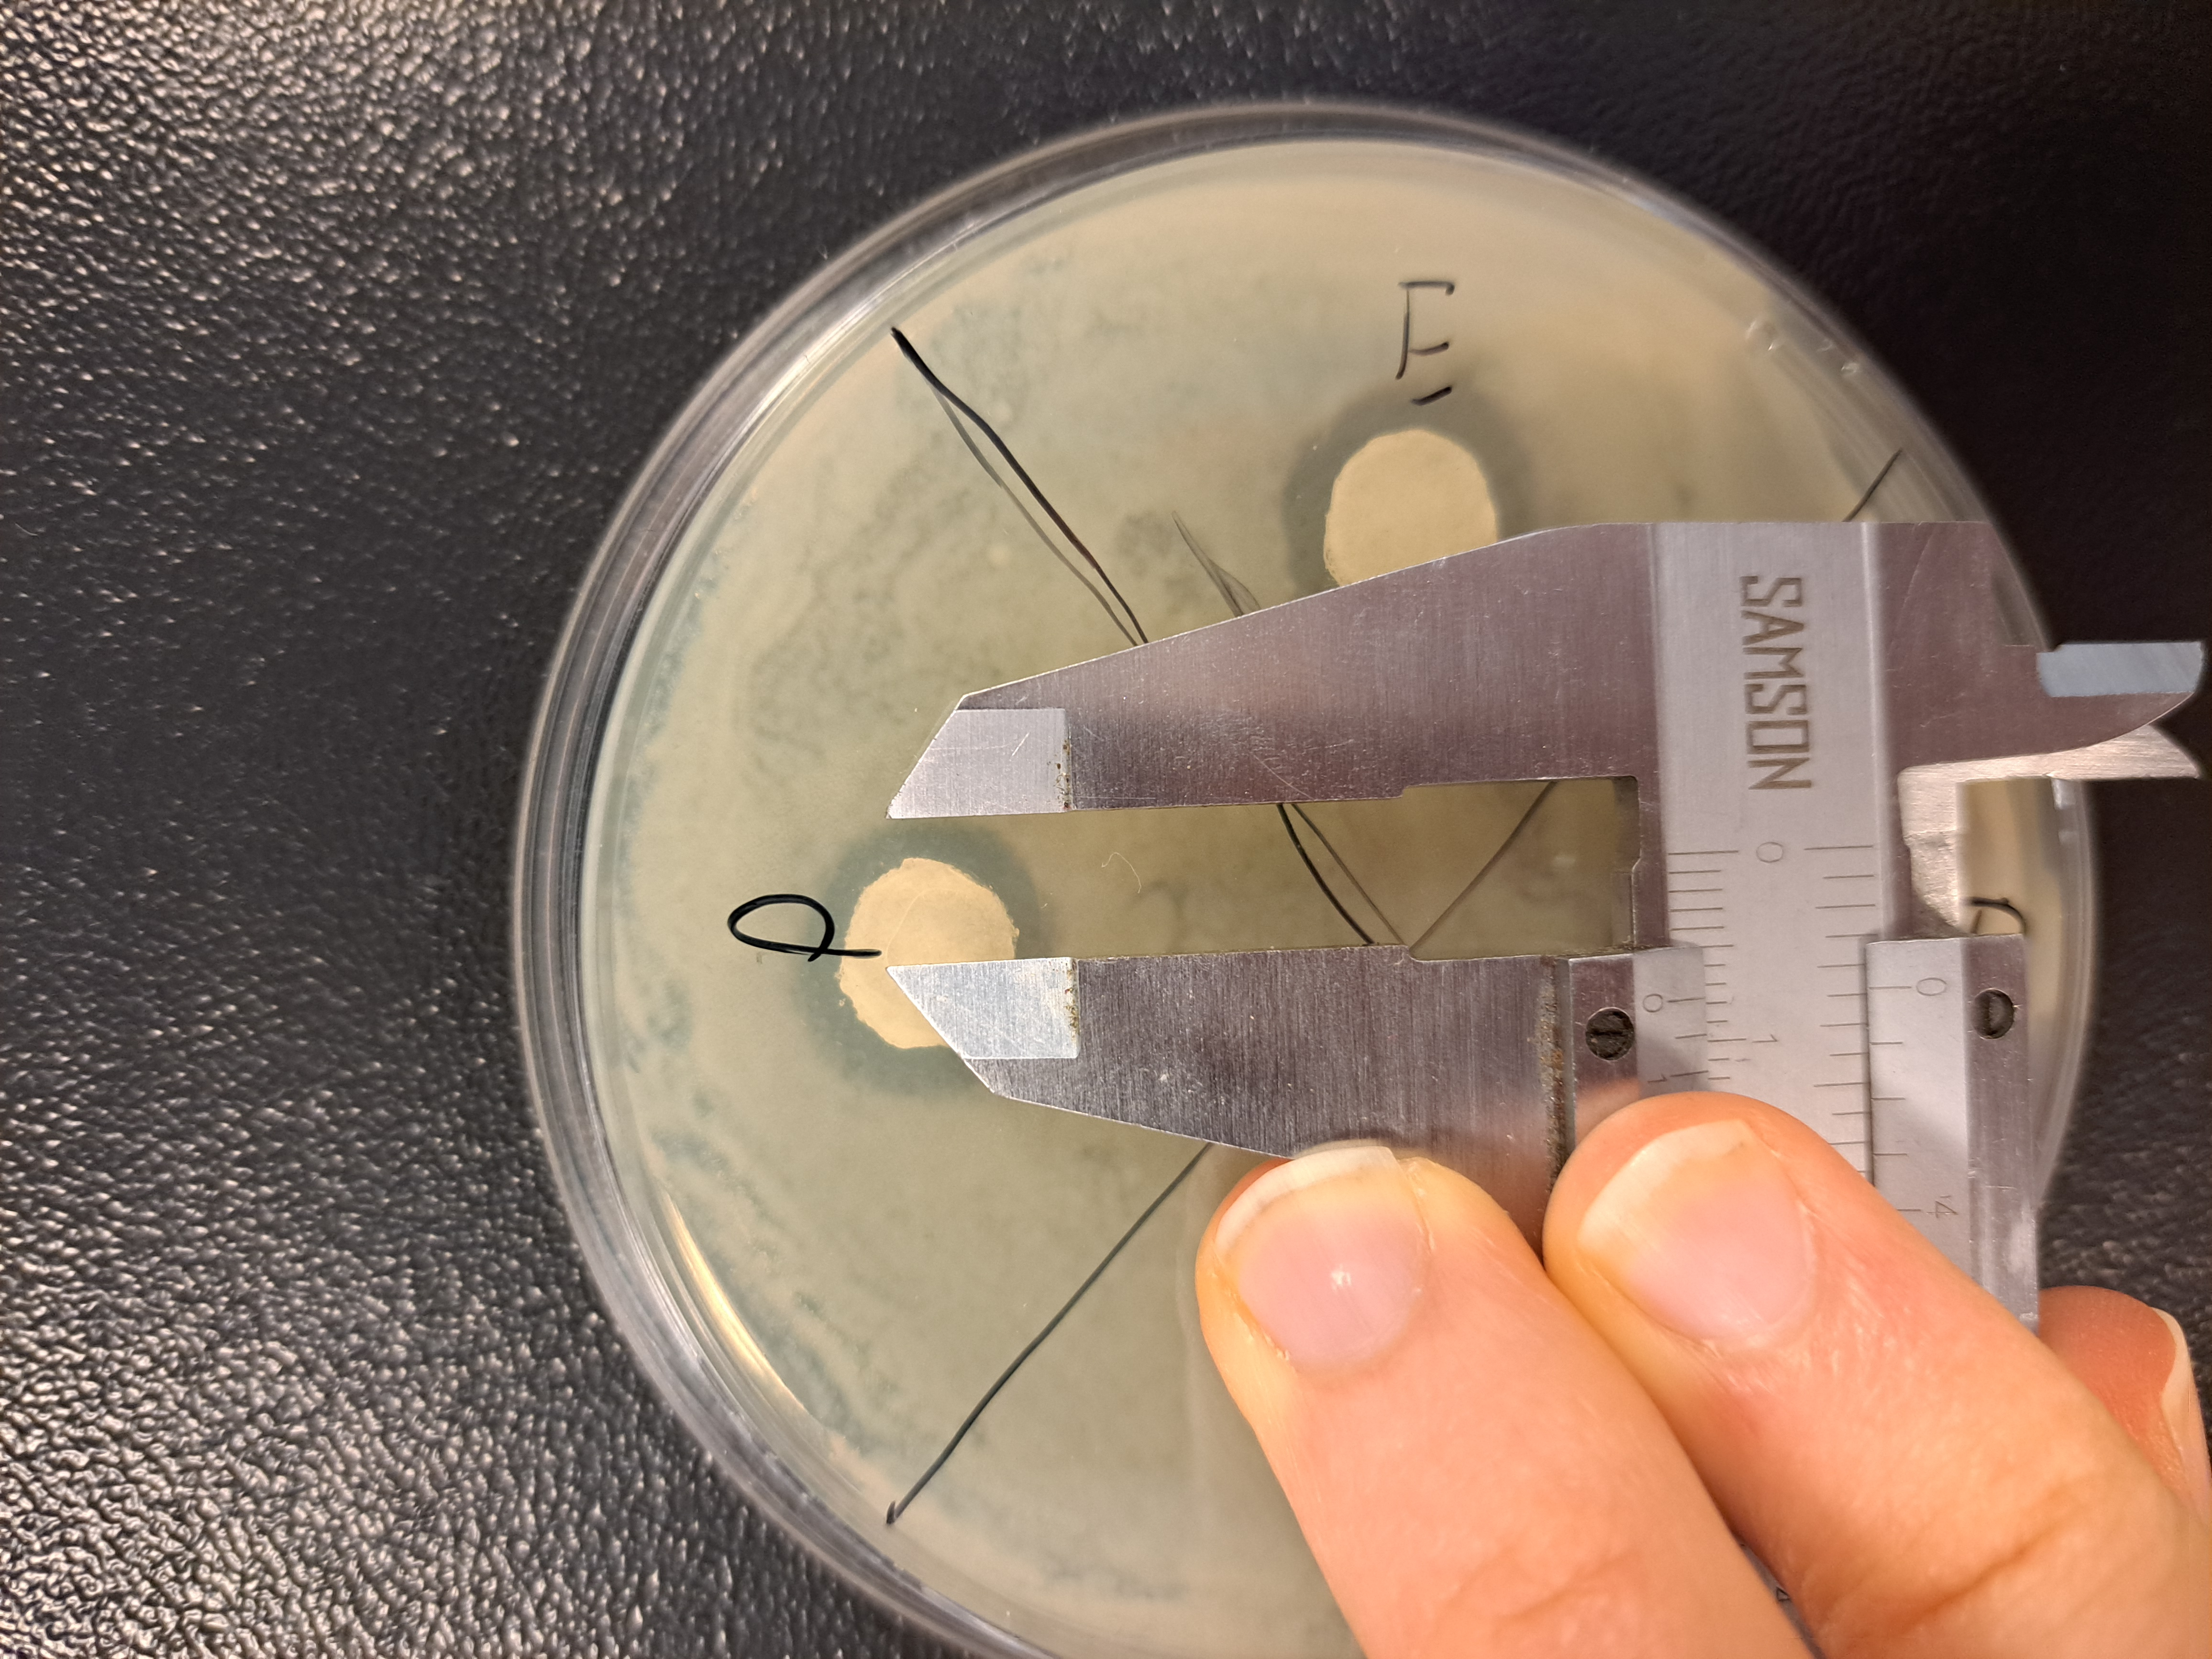
\includegraphics[width=.32\textwidth]{billeder/colip}
        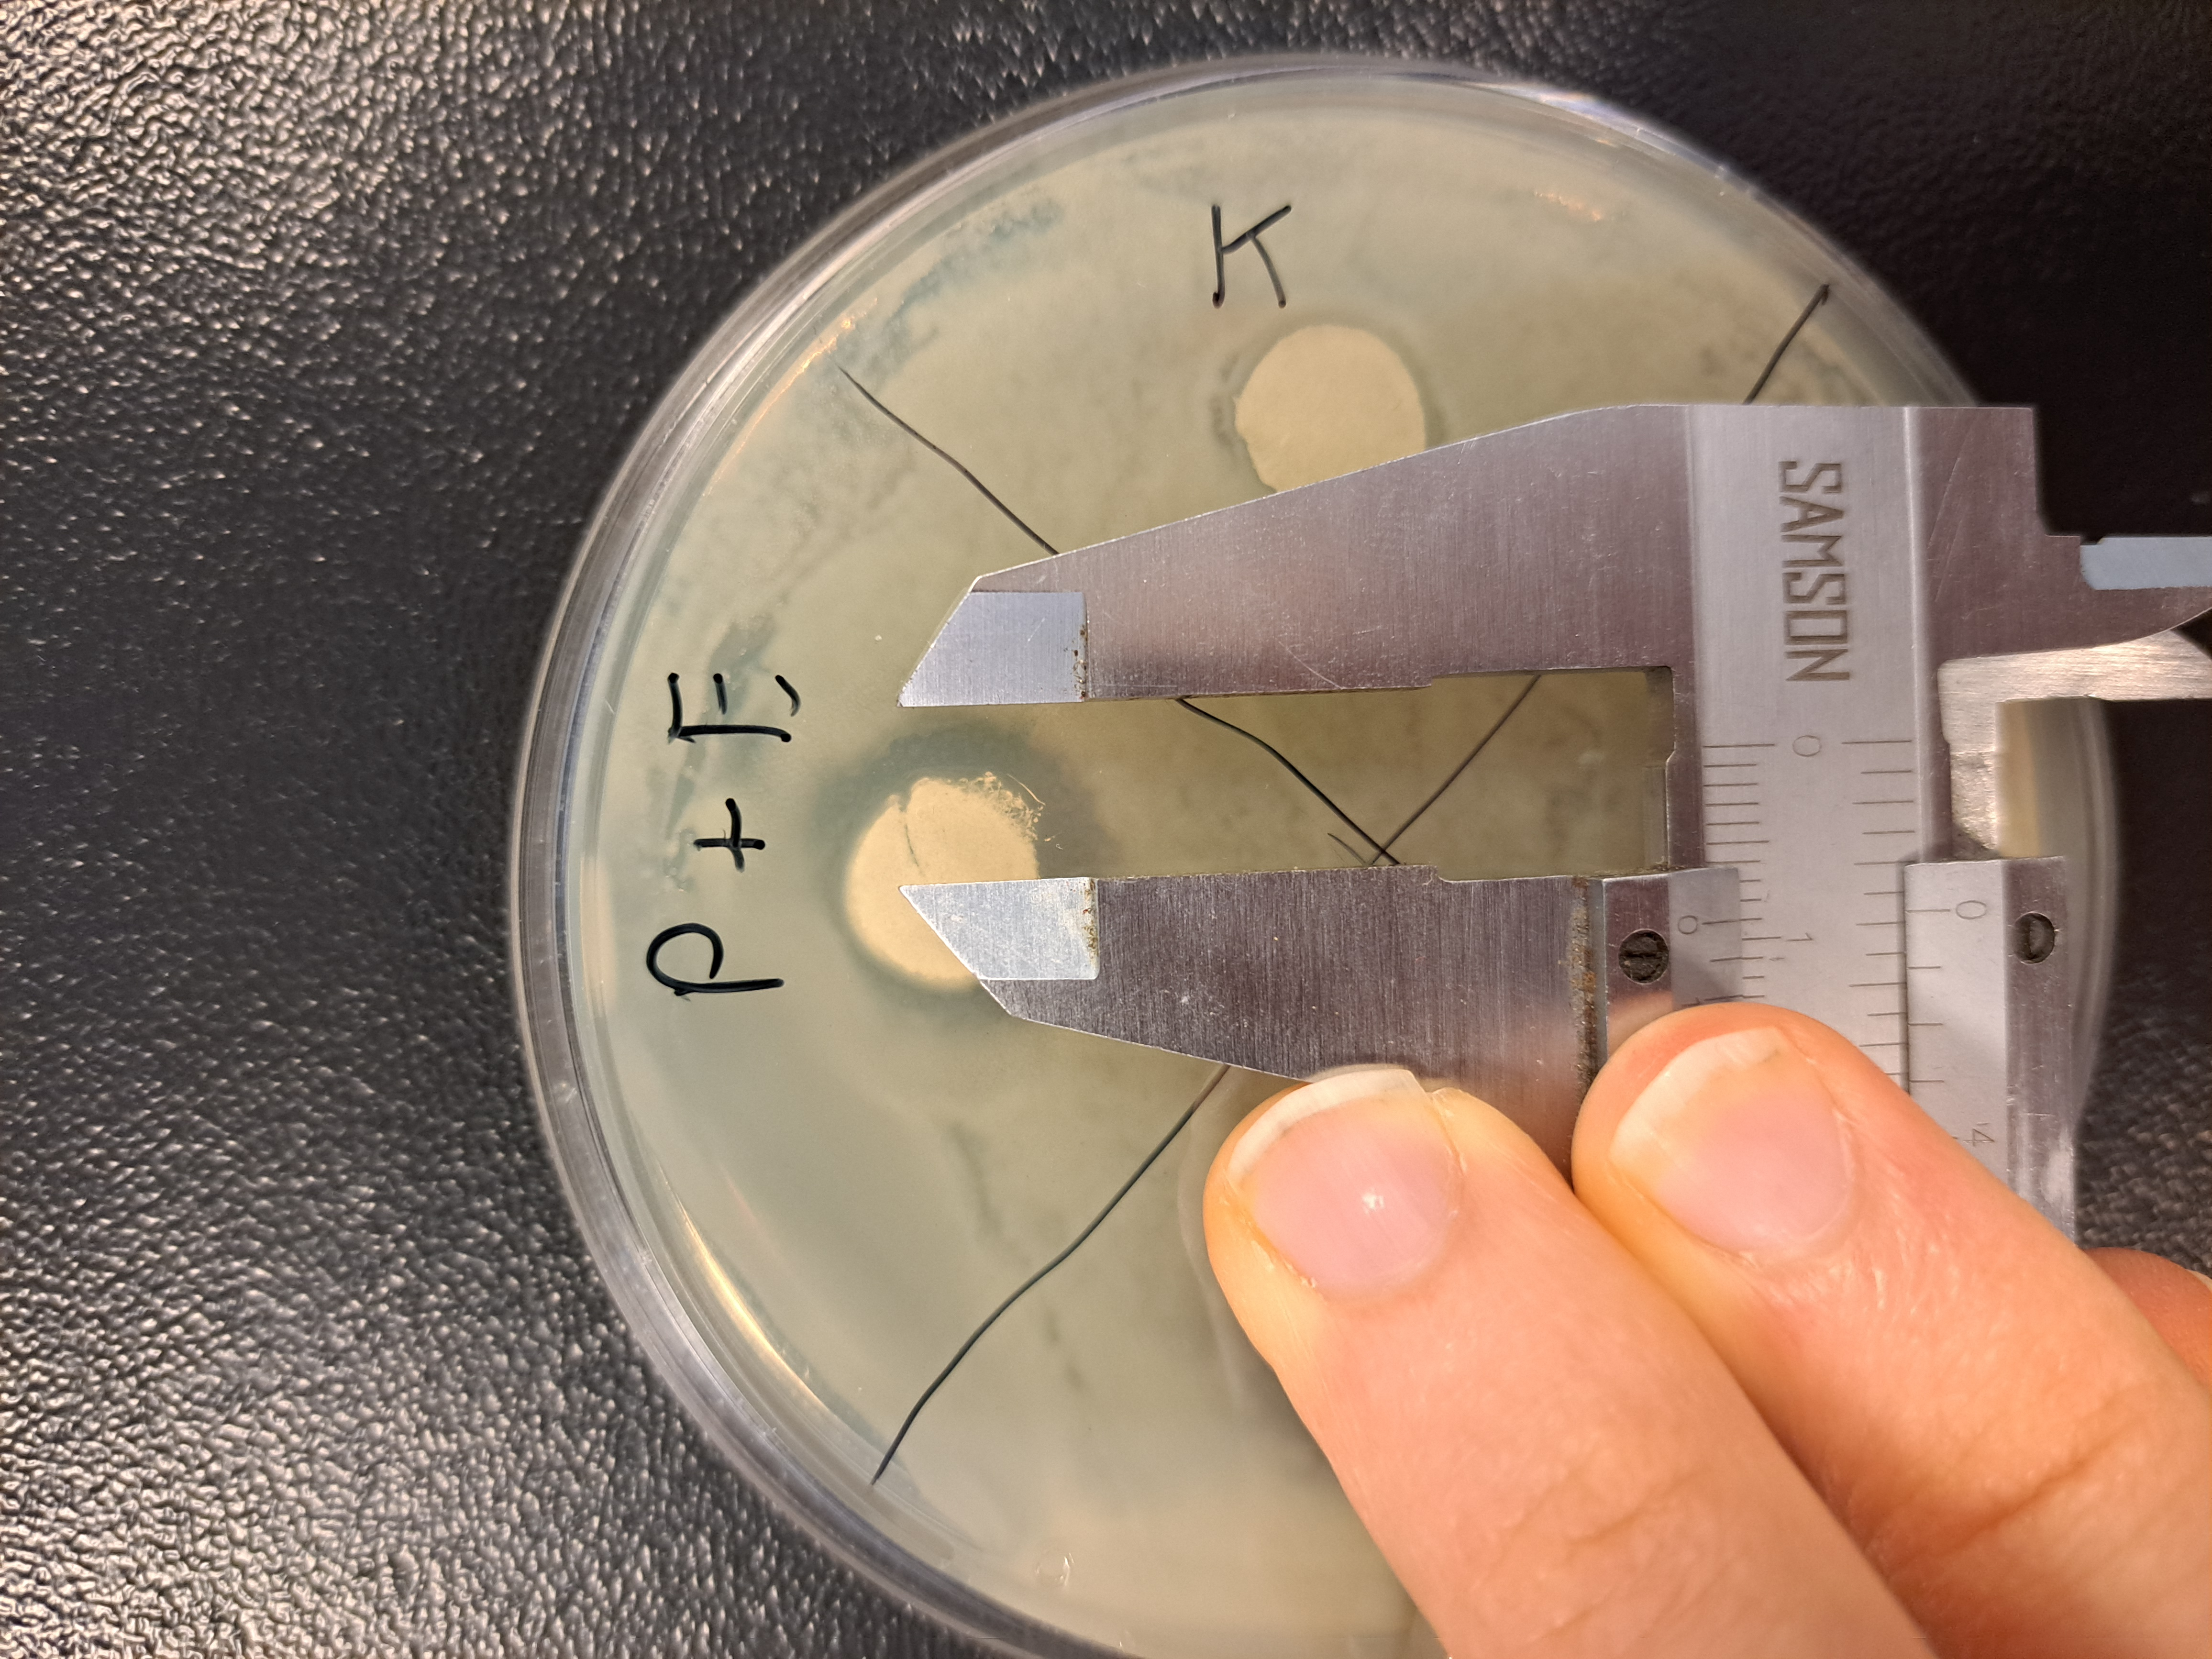
\includegraphics[width=.32\textwidth]{billeder/colipe}
        \caption{Hæmningsradier for colikolonien.}
    \end{figure}
    Ved aflæsning af hæmningsradierne får vi at:
    \begin{table}[H]\centering
        \caption{Hæmningsradier for \textit{bacillus cereus} og \textit{escherichia coli}.}
        \begin{tabular}{cccc}
            \toprule
            & \multicolumn{3}{c}{Hæmningsradius $\left[\si{cm}\right]$} \\
            \cmidrule(r){2-4}
            & Ethylparaben & Propylparaben & Blanding \\
            \midrule
            \textit{escherichia coli} & 0.75 & 0.77 & 0.90 \\
            \textit{bacillus cereus} & 0.70 & 0.79 & 0.82 \\
            \bottomrule
        \end{tabular}
    \end{table}
    Med udgangspunkt heri observeres konsekvent at blandingen er mere effektiv end propylparaben, som er mere effektiv end ethylparaben. For ethyl-- og propylparabenen giver dette giver også mening jf.\ teorien, da vi vil forvente at parabener med længere alkylkæder har en større hæmningseffekt. 
    
    For parabenblandingen kunne en mulig forklaring være at ethylparabenens større diffusionshastighed grundet mindre molekylestørrelse, samt større vandopløselighed, medierer større diffusion af propylparabenen ved at ``trække'' den med sig når den diffunderer, hvilket medfører at den mere potente propylparaben diffunderer en større afstand end i dens selvstændige test, hvilket lader den virke over et større område.
    
    Samtidigt giver dette også mulighed for at fremføre en hypotese om at MIC--værdien for propylparaben vil være lavere end ethylparaben under fortyndingsrækkeforsøget, hvilket passer med hvad vi har observeret i litteraturen.

    \subsubsection{Fortyndingsrække}
    Efter den 20 timer lange målingsperiode eksporteres dataene, og behandles for at være letforståelige. Til dette formål fremstilles en hhv.\ Abs(t)-- samt en Abs(c)--graf, der giver overblik over forløbet. Til fremstillingen af Abs(c)--grafen vælges det at benytte absorbansværdier fra $t=17\si{timer}$, da kontrollen lod til at nå den stationære fase her.
    \begin{figure}[H]\centering
        \includegraphics[width=.49\linewidth]{billeder/vækstbcethyl}
        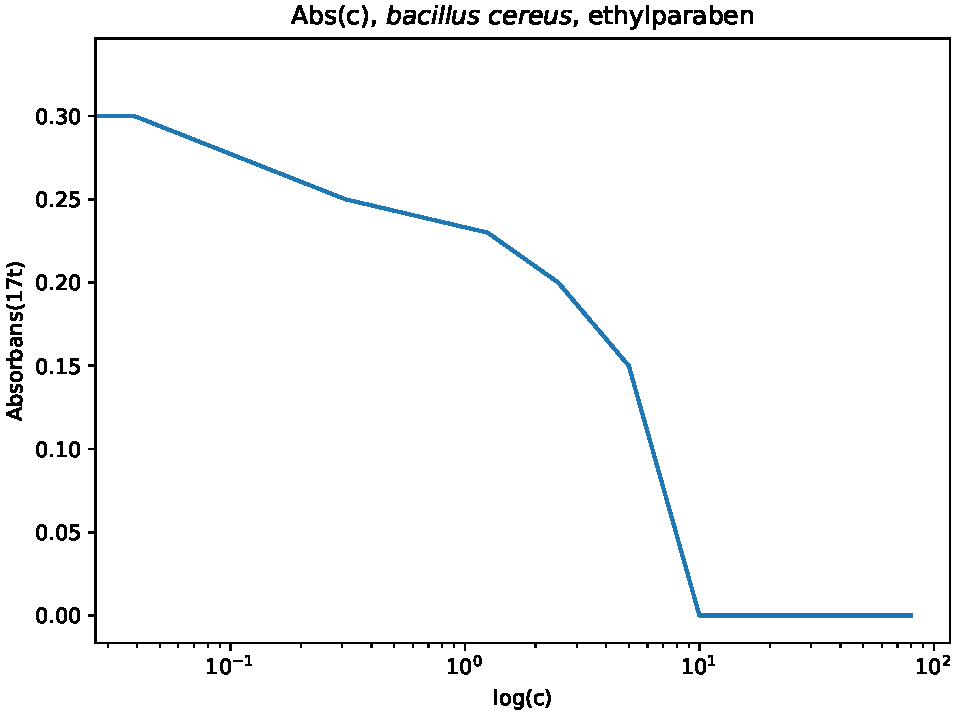
\includegraphics[width=.49\linewidth]{billeder/micbcethyl}
        \includegraphics[width=.49\linewidth]{billeder/vækstbcpropyl}
        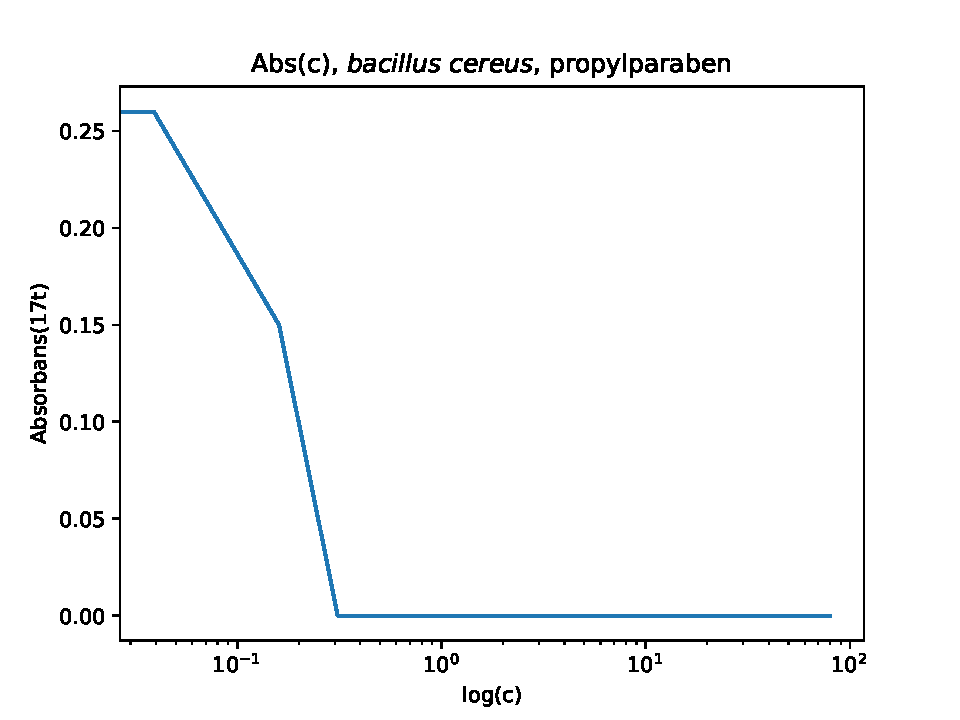
\includegraphics[width=.49\linewidth]{billeder/micbcpropyl}
        \caption{Abs(t)-- og Abs(c)--grafer for ethyl-- og propylparaben i medie poddet med \textit{bacillus cereus}. MIC--grafer er enkeltlogaritmiske.}
    \end{figure}
    Ved analyse af figuren er det klart at ethylparabenen havde en hæmmende effekt på mikroorganismerne uanset koncentration, idet alle de parabenholdige brønde endte med en lavere OD600 end kontrollen. Med udgangspunkt i Abs(c) grafen er det muligt at identificere cut--off punktet for forskellige MIC--værdier:
    \begin{table}[H]\centering
        \caption{MIC90, MIC50, MIC10, samt hæmningsintervallet for ethyl-- og propylparaben i \textit{bacillus cereus}--podet medie.}
        \begin{tabular}{ccccc}
            \toprule
            & \multicolumn{3}{c}{MIC $\left[\si{w\per w \%}\right]$} & \\
            \cmidrule(r){2-4}
            Paraben & MIC90 & MIC50 & MIC10 & Interval $\left[\si{w\per w \%}\right]$ \\
            \midrule
            Ethyl & 0.5--1 & 0.25--0.5 & 0.004--0.007 & $<0.004$--1 \\
            Propyl & 0.015--0.03 & 0.004--0.007 & $<0.004$ & $<0.004$--0.02 \\
            \bottomrule
        \end{tabular}
    \end{table}
    \begin{figure}[H]\centering
        \includegraphics[width=.48\linewidth]{billeder/vækstecethyl}
        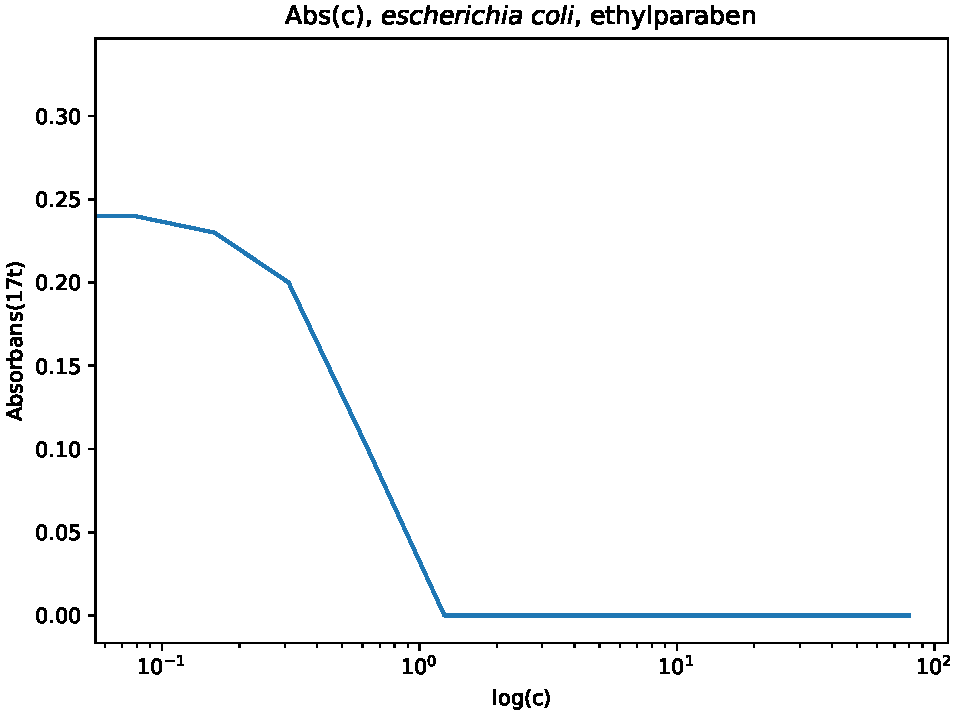
\includegraphics[width=.48\linewidth]{billeder/micecethyl}
        \includegraphics[width=.48\linewidth]{billeder/vækstecpropyl}
        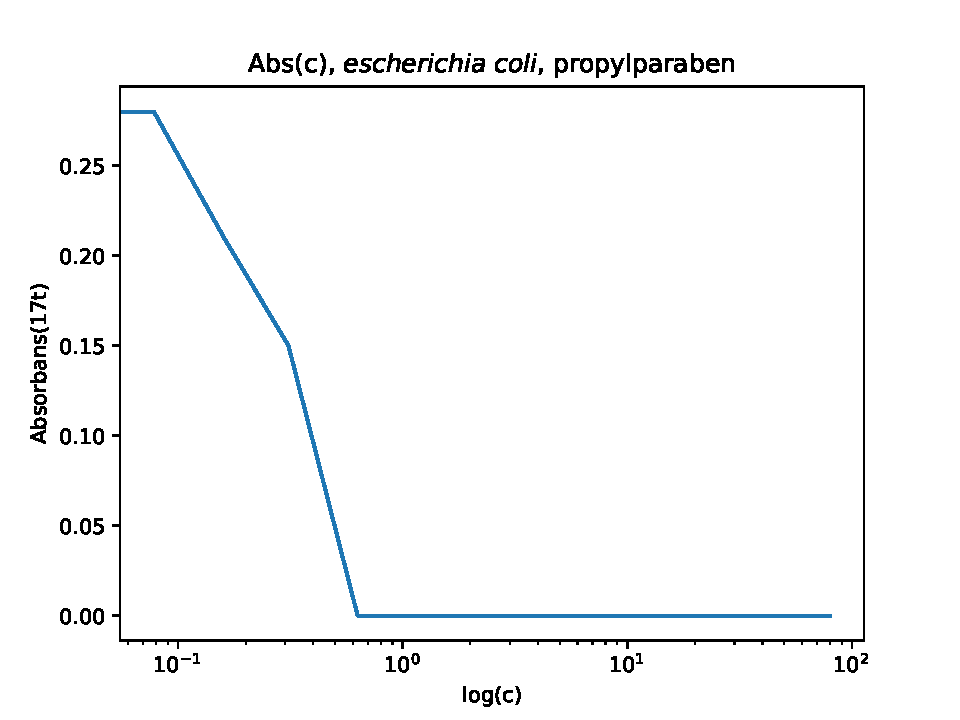
\includegraphics[width=.48\linewidth]{billeder/micecpropyl}
        \caption{Abs(t)-- samt Abs(c)--grafer for ethyl-- og propylparaben i medie poddet med \textit{eschericha coli}. MIC--grafer er enkeltlogaritmiske.}
    \end{figure}
    Her er det igen klart at der har været en konsekvent hæmmende effekt ved alle parabenkoncentrationer:
    \begin{table}[H]\centering
        \caption{MIC90, MIC50, MIC10, samt hæmningsintervallet for ethyl-- og propylparaben i \textit{escherichia coli}--podet medie.}
        \begin{tabular}{ccccc}
            \toprule
            & \multicolumn{3}{c}{MIC $\left[\si{w\per w \%}\right]$} & \\
            \cmidrule(r){2-4}
            Paraben & MIC90 & MIC50 & MIC10 & Interval $\left[\si{w\per w \%}\right]$ \\
            \midrule
            Ethyl & 0.06--0.125 & 0.03--0.06 & $<0.004$ & $<0.004$--0.125 \\
            Propyl & 0.03--0.06 & 0.015--0.03 & $<0.004$ & $<0.004$--0.06 \\
            \bottomrule
        \end{tabular}
    \end{table}
    Modsat litteraturen observeres her en tilsyneladende \textit{større} hæmningseffekt mod den gram--negative bakterieart end den gram--positive, hvilket vi umiddelbart ikke villet forvente. 

    En potentiel grund til dette kunnet være \textit{bacillus cereus'} evne til at danne et beskyttende biofilm \parencite{Joaq2020,Mich2021}, der kunnet have en skærmende effekt mod parabenernes virkning ved at gøre det sværere for dem at nå cellemembranen, bl.a.\ grundet dets høje vandindhold \parencite{Sati2023} som parabenerne villet være nødsaget til at bevæge sig gennem for at nå den lipide cellemembran. 

    \textit{Escherichia coli} har den samme egenskab \parencite{Chri2010}, dog er det muligt at den kemiske sammensætning af de dannede biofilm øger dets beskyttende effekt ved det dannet af \textit{bacillus cereus}. 

    Derudover er det også muligt at de kunnet have udviklet delvis antimikrobiel resistans, da analysen udførtes under den eksponentielle vækst--fase, hvilket muliggør hurtig evolution, og samhørigt tilpasning til dets miljø, hvilket kunnet indikere at \textit{bacillus cereus} har større kapacitet til at udvikle resistans overfor parabener. 

    Dette kunne igen muligvis kobles til dannelsen af biofilm, hvis fysiske egenskaber gennem evolutionen også kunnet ændre sig og gøre paraben--permeation endnu sværere.
